% !TeX spellcheck = it_IT
\documentclass{beamer}\usepackage[]{graphicx}\usepackage[]{color}
% maxwidth is the original width if it is less than linewidth
% otherwise use linewidth (to make sure the graphics do not exceed the margin)
\makeatletter
\def\maxwidth{ %
  \ifdim\Gin@nat@width>\linewidth
    \linewidth
  \else
    \Gin@nat@width
  \fi
}
\makeatother

\definecolor{fgcolor}{rgb}{0.345, 0.345, 0.345}
\newcommand{\hlnum}[1]{\textcolor[rgb]{0.686,0.059,0.569}{#1}}%
\newcommand{\hlstr}[1]{\textcolor[rgb]{0.192,0.494,0.8}{#1}}%
\newcommand{\hlcom}[1]{\textcolor[rgb]{0.678,0.584,0.686}{\textit{#1}}}%
\newcommand{\hlopt}[1]{\textcolor[rgb]{0,0,0}{#1}}%
\newcommand{\hlstd}[1]{\textcolor[rgb]{0.345,0.345,0.345}{#1}}%
\newcommand{\hlkwa}[1]{\textcolor[rgb]{0.161,0.373,0.58}{\textbf{#1}}}%
\newcommand{\hlkwb}[1]{\textcolor[rgb]{0.69,0.353,0.396}{#1}}%
\newcommand{\hlkwc}[1]{\textcolor[rgb]{0.333,0.667,0.333}{#1}}%
\newcommand{\hlkwd}[1]{\textcolor[rgb]{0.737,0.353,0.396}{\textbf{#1}}}%
\let\hlipl\hlkwb

\usepackage{framed}
\makeatletter
\newenvironment{kframe}{%
 \def\at@end@of@kframe{}%
 \ifinner\ifhmode%
  \def\at@end@of@kframe{\end{minipage}}%
  \begin{minipage}{\columnwidth}%
 \fi\fi%
 \def\FrameCommand##1{\hskip\@totalleftmargin \hskip-\fboxsep
 \colorbox{shadecolor}{##1}\hskip-\fboxsep
     % There is no \\@totalrightmargin, so:
     \hskip-\linewidth \hskip-\@totalleftmargin \hskip\columnwidth}%
 \MakeFramed {\advance\hsize-\width
   \@totalleftmargin\z@ \linewidth\hsize
   \@setminipage}}%
 {\par\unskip\endMakeFramed%
 \at@end@of@kframe}
\makeatother

\definecolor{shadecolor}{rgb}{.97, .97, .97}
\definecolor{messagecolor}{rgb}{0, 0, 0}
\definecolor{warningcolor}{rgb}{1, 0, 1}
\definecolor{errorcolor}{rgb}{1, 0, 0}
\newenvironment{knitrout}{}{} % an empty environment to be redefined in TeX

\usepackage{alltt}
\usepackage[]{graphicx}
\usepackage[]{color}

\usetheme{CambridgeUS}
\usecolortheme{seahorse}
%%%%%%%%%%%%%%%%%%%%%%%%%%%%%%%%%%%%%%%%%%%%%%%%%%%%%%%%%%%%%%%%%%5
%%  versione per stampa
%\documentclass[handout]{beamer}
\usepackage{pgfpages}
%\pgfpagesuselayout{8 on 1}[a4paper,border shrink=5mm,portrait]
%\usetheme{Pittsburgh}
%\usecolortheme{dove}

%\usecolortheme[RGB={60,165,222}]{structure} 
\usecolortheme[RGB={4,82,196}]{structure} 
\useoutertheme{modificatema}

%\setbeamercolor*{title}{fg=white,bg=gray!30!black}
\setbeamercolor*{frametitle}{parent=palette primary}

\setbeameroption{hide notes}

\usepackage{animate}
\usepackage[latin1]{inputenc}
\usepackage{epsfig}
\usepackage{boxedminipage}
\usepackage{multirow}
\usepackage{amsmath}
\usepackage{natbib}
\usepackage{verbatim}
%\usepackage{amssymb}
\usepackage{eepic}
\usepackage{amssymb}
\usepackage{color}
\usepackage[italian]{babel}
\setlength{\parindent}{0pt}
%\addtolength{\oddsidemargin}{-2cm}
%\addtolength{\evensidemargin}{-1cm}
%\addtolength{\textwidth}{3cm}
%\addtolength{\topmargin}{-5mm}
%\addtolength{\voffset}{-1cm}
%\addtolength{\textheight}{45mm}
\newcommand{\cov}{\ensuremath{\text{cov}}}
\newcommand{\var}{\ensuremath{\text{var}}}

\newcommand{\spa}{\vspace{3mm}\centerline{ *\hspace{1cm}*\hspace{1cm}*}\vspace{0.5cm}}

\newcommand{\tstim}{\ensuremath{\hat{\theta}}}
\newcommand{\tvero}{\ensuremath{\theta_0}}
\newcommand{\epsi}{\ensuremath{\varepsilon}}

\newcommand{\corr}[1]{{\textcolor{red}{#1}} }

\newcommand{\spaziobianco}{\vspace{2mm}}
\newcommand{\spazio}{\noindent\makebox[\linewidth]{\resizebox{0.1\linewidth}{1pt}{{$\bullet$}}}}

\newcommand{\thicksimH}{\overset{H_0}{\thicksim}}
\newcommand{\thicksimind}{\overset{\text{{\tiny IND}}}{\thicksim}}

\newcommand{\espon}[1]{\exp\left\{#1\right\}}

\newcommand{\N}[2]{\ensuremath{\mathcal N\left(#1,#2\right)}}
\newcommand{\Nbiv}[5]{\ensuremath{\mathcal N\left(\left[\begin{matrix}#1 \\ #2\end{matrix}\right],\left[\begin{matrix}#3 & #5 \\ #5 & #4\end{matrix}\right]\right)}}
\newcommand{\eps}{\ensuremath{\varepsilon}}

\setbeamercolor{verdescuro}{fg=structure!50!black,bg=white}
\setbeamercolor{titolo}{fg=white,bg=structure!50!black}
\setbeamercolor{corpo}{fg=black,bg=gray!20!white}


\usepackage{bm}

\newcommand{\vbeta}{\bm{\beta}}
\newcommand{\vb}{\bm{b}}
\newcommand{\vf}{\bm{f}}
\newcommand{\vu}{\bm{u}}
\newcommand{\vy}{\bm{y}}
\newcommand{\vx}{\bm{x}}
\newcommand{\veps}{\bm{\varepsilon}}
\definecolor{light-gray}{gray}{0.95}

\setbeamercolor{evidenzia}{fg=black,bg=yellow!20!white}


\setbeamertemplate{frametitle continuation}[from second][{\small}]
\beamertemplatenavigationsymbolsempty
\newenvironment{scatola}[1]{%
\begin{center}~%
\begin{beamerboxesrounded}[upper=titolo,lower=corpo,shadow=true,width=0.7\textwidth]{#1}}%
{%
\end{beamerboxesrounded}~%
\end{center}}

\newenvironment{scatolone}[1]{%
\begin{center}~%
\begin{beamerboxesrounded}[upper=titolo,lower=corpo,shadow=true,width=0.95\textwidth]{#1}}%
{%
\end{beamerboxesrounded}~%
\end{center}}

%\newenvironment{definizione}%
%{\vspace{3mm}{DEFINIZIONE,}\begin{it}}%
%{\end{it}\vspace{3mm}}

\newenvironment{definizione}%
{\vspace{3mm}\begin{scatola}{Definizione}}%
{\end{scatola}\vspace{3mm}}

\newenvironment{teorema}%
{\vspace{3mm}\begin{scatola}{Teorema}}%
{\end{scatola}\vspace{3mm}}

\newenvironment{proprieta}%
{\vspace{3mm}\begin{scatola}{Propriet\`a}}%
{\end{scatola}\vspace{3mm}}


%\newcounter{nteo}
%\newenvironment{teorema}%
%{\vspace{3mm}{TEOREMA,}\begin{it}}%
%{\end{it}\vspace{3mm}}

%%\newcounter{nprop}
%\newenvironment{proprieta}%
%{\vspace{3mm}{PROPRIET\`A,}\begin{it}}%
%{\end{it}\vspace{3mm}}

\usepackage{bm}

\newcounter{nlucido}

%\author[ Trieste, 7 marzo 2012, lucido \thenlucido]{FP AS SZ}

\title[Regressione semiparametrica]{5. Regressione semiparametrica}

\author[F. Pauli]{Francesco Pauli}


\institute{DEAMS \\ Universit\`a di Trieste}

\date{A.A. 2017/2018}

\AtBeginSection[] % Do nothing for \section*
{
\begin{frame}
\frametitle{Indice}
\tableofcontents[currentsection,hideallsubsections]
%\tableofcontents[currentsection]
\end{frame}
}
\AtBeginSubsection[] % Do nothing for \section*
{
\begin{frame}<beamer>
\frametitle{Indice}
\tableofcontents[sectionstyle=show/shaded,subsectionstyle=show/shaded/hide]
%\tableofcontents[currentsection,currentsubsection]
\end{frame}
}
\IfFileExists{upquote.sty}{\usepackage{upquote}}{}
\IfFileExists{upquote.sty}{\usepackage{upquote}}{}
\begin{document}
\SweaveOpts{concordance=TRUE}

%\input{richiami}




\maketitle
%\input{traccia}




\begin{frame}{Modelli parametrici, semiparametrici, non parametrici}
Si ha un modello parametrico quando la famiglia di distribuzioni all'-interno della quale cerchiamo una distribuzione che descriva i dati \`e indicizzata da un parametro $\theta\in\mathbb R^d$, \textbf{con $d$ non troppo grande e fisso}.

\spazio

Muoversi verso i metodi semiparametrici o non parametrici significa
\begin{itemize}
\item ridurre le assunzioni
\item aumentare il numero di parametri e, in qualche senso, stimarlo
\end{itemize}
(non c'\`e una separazione netta).

\spazio

\onslide*<1>{
Esempio: stima della distribuzione di $X_1,\ldots,X_n\thicksim F()$
\begin{itemize}
\item parametrica: si assume $F\in\mathcal F=\{F_\theta():\theta\in\mathbb R^d\}$, si stima $\theta$ (ad es. SMV),  $F_{\hat{\theta}}$ \`e la stima di $F$.
\item non parametrica: si assume $F$ sia una FdR: una buona stima \`e la {\bf FdR empirica}.
\end{itemize}
}
\onslide*<2>{
Esempio: stima della funzione di regressione $E(Y|X=x)$ da un campione $(x_i,Y_i)$, $i=1,\ldots,n$
\begin{itemize}
\item parametrica: si assume $E(Y|X=x)=\beta_1+\beta_2x$, si stima $\theta=(\beta_1,\beta_2)$.
\item non parametrica: si assume $E(Y|X=x)=f(x)$  dove $f$ appartiene a una classe di funzioni sufficientemente flessibile (non ci sono parametri di interesse diretto).
\end{itemize}
}

\end{frame}


\begin{frame}[t]{Regressione non parametrica}
Si assume che
\[ E(Y|X= x) = f(x);\;\;\; V(Y|X=x)=\sigma^2   \]
dove $f$ \`e una funzione ``regolare'' (continua con qualche derivata continua).

\spazio

Due approcci
\begin{itemize}
\item tecniche ``locali''%
\onslide*<1>{%
\begin{itemize}
\item se avessimo tante osservazioni per ciascun $x_0$ potremmo stimare $f(x_0)$ come una media campionaria.
\item in generale, avendo un'osservazione per ciascun $x$ potremmo usare le osservazioni vicine.
\end{itemize}
}%
\onslide*<2->{: stima $E(Y|X=x_0)$ usando punti vicini a $x_0$.}
\onslide*<2->{
\item tecniche ``globali''  (spline)%
}%
\onslide*<3->{%
: definiamo un modello flessibile per $f(x;{\bm\theta})$
}%
\onslide*<2>{
\begin{itemize}
\item definiamo una classe di funzioni $f(x;{\bm\theta})$ abbastanza flessibile da poter approssimare qualunque funzione regolare $f(\cdot)$
\item stimiamo  $f$ scegliendo il miglio rappresentante in $f(x;{\bm\theta})$
\end{itemize}
}
\end{itemize}
\onslide*<4->{
Un aspetto cruciale in entrambi i metodi \`e determinare quanto liscia debba essere $\hat{f}$ che si traduce in 
\begin{itemize}
\item decidere cosa significa ``vicino''
\item decidere quanto flessibile dev'essere il modello $f(x;{\bm\theta})$ 
\end{itemize}
In entrambi i casi, serve un compromesso tra distorsione e varianza.
}
\end{frame}



\section[Gaussiana]{Regressione non parametrica, caso gaussiano}


\begin{knitrout}
\definecolor{shadecolor}{rgb}{0.969, 0.969, 0.969}\color{fgcolor}\begin{kframe}


{\ttfamily\noindent\color{warningcolor}{Warning in file(file, "{}rt"{}): cannot open file 'wmap.dat': No such file or directory}}

{\ttfamily\noindent\bfseries\color{errorcolor}{Error in file(file, "{}rt"{}): non posso aprire questa connessione}}

{\ttfamily\noindent\color{warningcolor}{Warning in file(file, "{}rt"{}): cannot open file 'lidar.dat': No such file or directory}}

{\ttfamily\noindent\bfseries\color{errorcolor}{Error in file(file, "{}rt"{}): non posso aprire questa connessione}}

{\ttfamily\noindent\bfseries\color{errorcolor}{Error in eval(expr, envir, enclos): oggetto "{}lidar"{} non trovato}}

{\ttfamily\noindent\color{warningcolor}{Warning in file(file, "{}rt"{}): cannot open file 'bpd.dat': No such file or directory}}

{\ttfamily\noindent\bfseries\color{errorcolor}{Error in file(file, "{}rt"{}): non posso aprire questa connessione}}\end{kframe}
\end{knitrout}


\begin{frame}[fragile]{Esempio: dati ``lidar''}
\begin{columns}
\column{0.45\textwidth}
\begin{knitrout}
\definecolor{shadecolor}{rgb}{0.969, 0.969, 0.969}\color{fgcolor}\begin{kframe}


{\ttfamily\noindent\bfseries\color{errorcolor}{Error in plot(lidar\$range, lidar\$logratio, pch = 20, xlab = "{}range (standardized)"{}, : oggetto "{}lidar"{} non trovato}}\end{kframe}
\end{knitrout}
\column{0.55\textwidth}
LIDAR = LIght Detection And Ranging
\begin{itemize}
\item \`e una tecnica per individuare composti chimici nell'atmosfera
\item $x$: distanza percorsa prima della riflessione
\item $y$: logaritmo del rapporto tra luce ricevuta tra le due fonti laser
\end{itemize}
\end{columns}

\begin{itemize}
\item L'obiettivo \`e stimare
\[ f(x) = E(Y|X=x) \]
\item
(Esempio ben noto dove le tecniche banali, trasformazioni o regressione polinomiale, funzionano male.)
\end{itemize}
\end{frame}



\begin{frame}[t]{LIDAR: modello lineare}
\begin{columns}[T]
\column{0.5\textwidth}
Assumiamo
\[ {\bf y} = X{\bm\beta} + {\bm\varepsilon} \]
dove $X\in\mathcal M_{n\times p}$, ${\bm\beta}\in\mathbb R^p$, ${\bm\varepsilon}\thicksim N(0,\sigma^2I)$, 
\begin{knitrout}
\definecolor{shadecolor}{rgb}{0.969, 0.969, 0.969}\color{fgcolor}\begin{kframe}


{\ttfamily\noindent\bfseries\color{errorcolor}{Error in plot(lidar\$range, lidar\$logratio, pch = 20, xlab = "{}x"{}, ylab = "{}y"{}, : oggetto "{}lidar"{} non trovato}}

{\ttfamily\noindent\bfseries\color{errorcolor}{Error in eval(predvars, data, env): oggetto "{}lidar"{} non trovato}}\end{kframe}
\end{knitrout}

Non molto soddisfacente...
\column{0.5\textwidth}
\onslide*<1>{
Usando la massima verosimiglianza
\[ {\hat{\bm\beta}} = (X^TX)^{-1}X^T{\bf y} \]
sicch\'e
\[ {\bf\hat y} = X{\hat{\bm\beta}}= X(X^TX)^{-1}X^T{\bf y} \]
dove $H=X(X^TX)^{-1}X^T$ \`e la matrice di proiezione da $\mathbb R^n$ al sottospazio generato dalle colonne di $X$, si ricordi che
\[ \mbox{trace}{H}=p \]
}
\onslide*<2>{
Si noti che
\[ {\bf\hat y} = X{\hat{\bm\beta}}{\bf y}= X(X^TX)^{-1}X^T{\bf y} \]
significa che la stima del valore atteso condizionato \`e
\[ \widehat{E(Y|X=x)} = \hat{f}(x) = \sum_{i=1}^n h_i(x) Y_i \]
dove
\[ h({\bf x})^T= {\bf x}^T(X^TX)^{-1}X^T \]
}
\end{columns}
\end{frame}



\begin{frame}{LIDAR: costante a tratti}
Consideriamo una partizione dello spazio della variabile esplicativa, indichiamo gli estremi degli intervalli con
\[ -\infty= c_0 < c_1 < \ldots < c_{K-1} < c_K = +\infty \]
\begin{columns}[T]
\column{0.5\textwidth}
\begin{knitrout}
\definecolor{shadecolor}{rgb}{0.969, 0.969, 0.969}\color{fgcolor}\begin{kframe}


{\ttfamily\noindent\bfseries\color{errorcolor}{Error in eval(expr, envir, enclos): oggetto "{}lidar"{} non trovato}}

{\ttfamily\noindent\bfseries\color{errorcolor}{Error in eval(expr, envir, enclos): oggetto "{}lidar"{} non trovato}}

{\ttfamily\noindent\bfseries\color{errorcolor}{Error in eval(expr, envir, enclos): oggetto "{}x"{} non trovato}}

{\ttfamily\noindent\bfseries\color{errorcolor}{Error in plot(lidar\$range, lidar\$logratio, pch = 20, xlab = "{}x"{}, ylab = "{}y"{}): oggetto "{}lidar"{} non trovato}}

{\ttfamily\noindent\bfseries\color{errorcolor}{Error in int\_abline(a = a, b = b, h = h, v = v, untf = untf, ...): plot.new has not been called yet}}

{\ttfamily\noindent\bfseries\color{errorcolor}{Error in eval(expr, envir, enclos): oggetto "{}y"{} non trovato}}

{\ttfamily\noindent\bfseries\color{errorcolor}{Error in lines(x[(x >= c[i]) \& (x < c[i + 1])], rep(mean(y[(x >= c[i]) \& : oggetto "{}x"{} non trovato}}\end{kframe}
\end{knitrout}
\column{0.5\textwidth}
e stimiamo $E(Y|X=x)$ assumendo sia costante negli intervalli
\[ \hat{f}(x) = \frac{\sum_{k=0}^{K-1}\sum_{i=1}^n y_i I_{[c_k,c_{k+1}]}(x_i)}{\sum_{k=0}^{K-1}\sum_{i=1}^n I_{[c_k,c_{k+1}]}(x_i)} \]

Il risultato 
\begin{itemize}
\item non \`e liscio (addirittura discontinuo), e 
\item dipende dalla scelta degli intervalli.
\end{itemize}
\end{columns}

\end{frame}


\begin{frame}[t]{LIDAR: media mobile\onslide*<2>{ (vicini pi\`u vicini)}}
Se assumiamo che $f(x)$ sia continua, allora \`e ragionevole stimare $f(x)$ come la media di valori di  $Y_i$ che corrispondono a $x_i$ vicini a $x$.
\begin{columns}[T]
\column{0.5\textwidth}
\onslide*<1>{
\begin{knitrout}
\definecolor{shadecolor}{rgb}{0.969, 0.969, 0.969}\color{fgcolor}\begin{kframe}


{\ttfamily\noindent\bfseries\color{errorcolor}{Error in plot(lidar\$range, lidar\$logratio, pch = 20, xlab = "{}x"{}, ylab = "{}y"{}): oggetto "{}lidar"{} non trovato}}

{\ttfamily\noindent\bfseries\color{errorcolor}{Error in mapply(runmean, x, MoreArgs = list(xx = xx, yy = yy, h = h)): oggetto "{}lidar"{} non trovato}}

{\ttfamily\noindent\bfseries\color{errorcolor}{Error in mapply(runmean, x, MoreArgs = list(xx = xx, yy = yy, h = h)): oggetto "{}lidar"{} non trovato}}

{\ttfamily\noindent\bfseries\color{errorcolor}{Error in strwidth(legend, units = "{}user"{}, cex = cex, font = text.font): plot.new has not been called yet}}\end{kframe}
\end{knitrout}

}
\onslide*<2>{
\begin{knitrout}
\definecolor{shadecolor}{rgb}{0.969, 0.969, 0.969}\color{fgcolor}\begin{kframe}


{\ttfamily\noindent\bfseries\color{errorcolor}{Error in plot(lidar\$range, lidar\$logratio, pch = 20, xlab = "{}x"{}, ylab = "{}y"{}): oggetto "{}lidar"{} non trovato}}

{\ttfamily\noindent\bfseries\color{errorcolor}{Error in mapply(hneighmean, x, MoreArgs = list(xx = xx, yy = yy, h = h)): oggetto "{}lidar"{} non trovato}}

{\ttfamily\noindent\bfseries\color{errorcolor}{Error in mapply(hneighmean, x, MoreArgs = list(xx = xx, yy = yy, h = h)): oggetto "{}lidar"{} non trovato}}

{\ttfamily\noindent\bfseries\color{errorcolor}{Error in strwidth(legend, units = "{}user"{}, cex = cex, font = text.font): plot.new has not been called yet}}\end{kframe}
\end{knitrout}

}
\column{0.5\textwidth}
\onslide*<1>{

In particulare potremmo usare la media di quegli $x_i$ che giacciono in un intorno di $x$ di raggio $h$
\[ \hat{f}(x) = \frac{\sum_{i=1}^n y_i I_{h}(|x-x_i|)}{\sum_{i=1}^n I_{h}(|x-x_i|)} \]

}

\onslide<2>{
Alternativamente potremmo usare la media dei $k$ vicini pi\`u vicini ad $x$, 
\[ N_k(x)=\{x_i: |x-x_i|\leq d_{(k)}\} \]
dove $d_i=|x-x_i|$ e $d_{(1)}\leq \ldots\leq d_{(n)}$ sono le distanze ordinate, allora
\[ \hat{f}(x) = \frac{1}{k} \sum_{i=1}^n y_i I_{N_k(x)}(x_i) \]

}
\end{columns}

\end{frame}




\begin{frame}{Errore di stima: distorsione e varianza}
La stima
\[ \hat{f}(x) = \frac{1}{k} \sum_{i=1}^n y_i I_{N_k(x)}(x_i)  
= \frac{1}{k} \sum_{y_i\in N_k(x)} y_i  \]
dove $N_k(x)=\{x_i: |x-x_i|\leq d_{(k)}\}$ \`e basata su  $k$ osservazioni: {\bf pi\`u grande \`e $k$}, 
\begin{itemize}
\item pi\`u osservazioni sono usate e quindi minore \`e la variabilit\`a:
\begin{itemize}
\item<2>  {\bf pi\`u piccola \`e la  varianza}
\end{itemize}
\item d'altra parte, s'impiegano osservazioni pi\`u distanti, a seconda della forma di $f()$ in un intorno di $x$, la media delle osservazioni pu\`o differire pi\`u o meno marcatamente da $E(Y|X=x)=f(x)$:
\begin{itemize}
\item<2>  {\bf pi\`u grande \`e la distorsione}
\end{itemize}
\end{itemize}
Il compromesso tra distorsione e varianza \`e una caratteristica distintiva dei lisciatori.
\end{frame}

\begin{frame}{Distorsione, forma di $f$ e $k$}
\begin{knitrout}
\definecolor{shadecolor}{rgb}{0.969, 0.969, 0.969}\color{fgcolor}
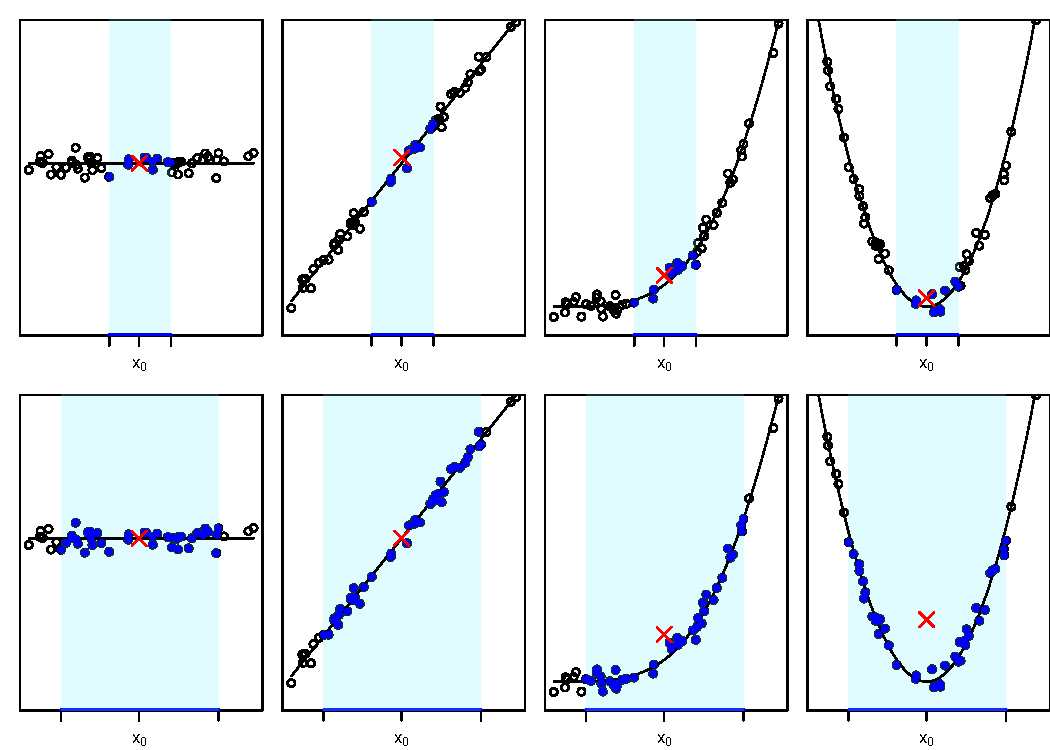
\includegraphics[width=0.9\textwidth]{figure/020-regression-1unnamed-chunk-6-1} 

\end{knitrout}
\end{frame}

\begin{frame}[t]{Derivazione teorica di distorsione e varianza}
Sia $N_k(x)=\{x_i: |x-x_i|\leq d_{(k)}\}$, e lo stimatore 
\[ \hat{f}(x) = \frac{1}{k} \sum_{i=1}^n y_i I_{N_k(x)}(x_i) = \frac{1}{k} \sum_{y_i\in N_k(x)} y_i \]


\onslide*<1>{
La varianza \`e (assumendo $V(Y_i)=\sigma^2$ per ogni $i$)
\[ V(\hat{f}(x)) = \frac{1}{k}\sum_{y_i\in N_k(x)}V(Y_i) = \frac{\sigma^2}{k} \]
}
\onslide*<2>{
La distorsione \`e
\begin{align*}
E(\hat{f}(x))-f(x) 
&= \frac{1}{k} \sum_{N_k(x)} (f(x_i)-f(x)) \\
&\approx \frac{1}{k} \sum_{N_k(x)} \left(f'(x)(x_i-x)+\frac{1}{2}f''(x)(x_i-x)^2\right) \\
\intertext{assumendo le covariate equidistanziate: $x_{i+1}-x_i=\Delta$}
&\approx  \frac{2k(k+2)(k+1)}{6k} f''(x)\Delta^2
\end{align*}
}
\onslide*<3>{
Quindi l'MSE \`e
\[ E((\hat{f}(x)-f(x))^2) \approx \left(\underbrace{\frac{2k(k+2)(k+1)}{6k} f''(x)\Delta^2 }_{distorsione}\right)^2 + \underbrace{\frac{\sigma^2}{k}}_{varianza}\]
e quindi
\begin{itemize}
\item la distorsione cresce con $k$ e con $|f''|$
\item la varianza decresce con $k$
\end{itemize}
}
\end{frame}



\begin{frame}[t]{Distorsione e varianza, esempio}
Consideriamo un campione, la vera $f(\cdot)$ \`e in verde, 
\onslide<2->{
\begin{itemize}
\item calcoliamo distorsione, varianza e quindi MSE per $\hat{f}_k(0.6)$ in funzione di $k$, individuiamo un valore ottimale di $k$.
\onslide<3>{
\item facciamo lo stesso per $\hat{f}_k(0.9)$, otteniamo un {\bf diverso} valore ottimale di $k$.
}
\end{itemize}
} 

\begin{columns}[T]
\column{0.33\textwidth}
\onslide*<1>{%
\begin{knitrout}
\definecolor{shadecolor}{rgb}{0.969, 0.969, 0.969}\color{fgcolor}
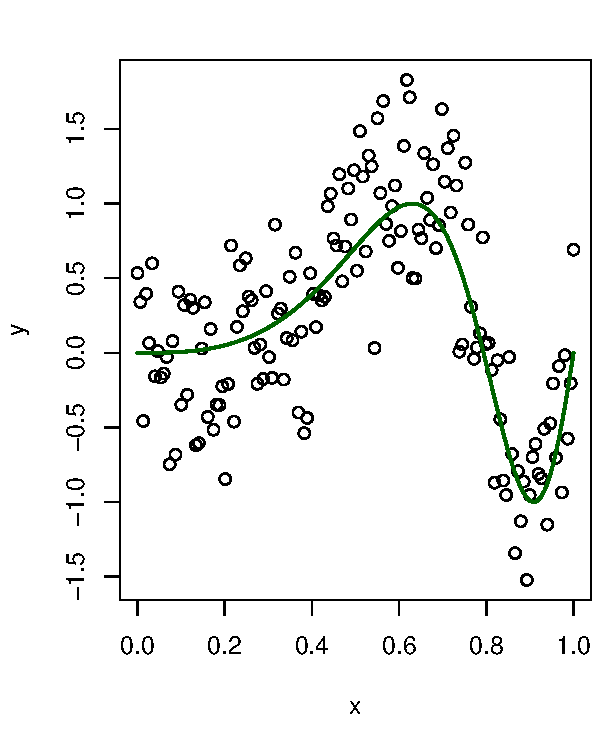
\includegraphics[width=0.95\textwidth]{figure/020-regression-1unnamed-chunk-8-1} 

\end{knitrout}
}%
\onslide*<2>{%
\begin{knitrout}
\definecolor{shadecolor}{rgb}{0.969, 0.969, 0.969}\color{fgcolor}
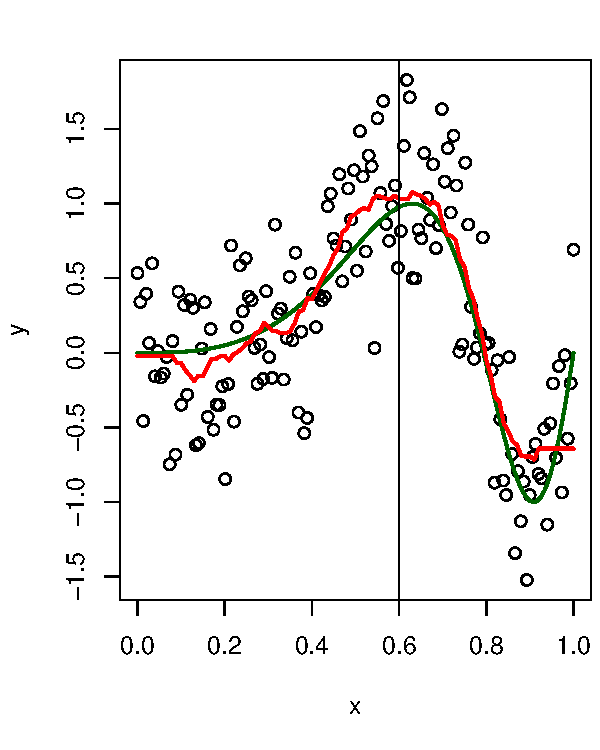
\includegraphics[width=0.95\textwidth]{figure/020-regression-1unnamed-chunk-9-1} 

\end{knitrout}
}%
\onslide*<3>{%
\begin{knitrout}
\definecolor{shadecolor}{rgb}{0.969, 0.969, 0.969}\color{fgcolor}
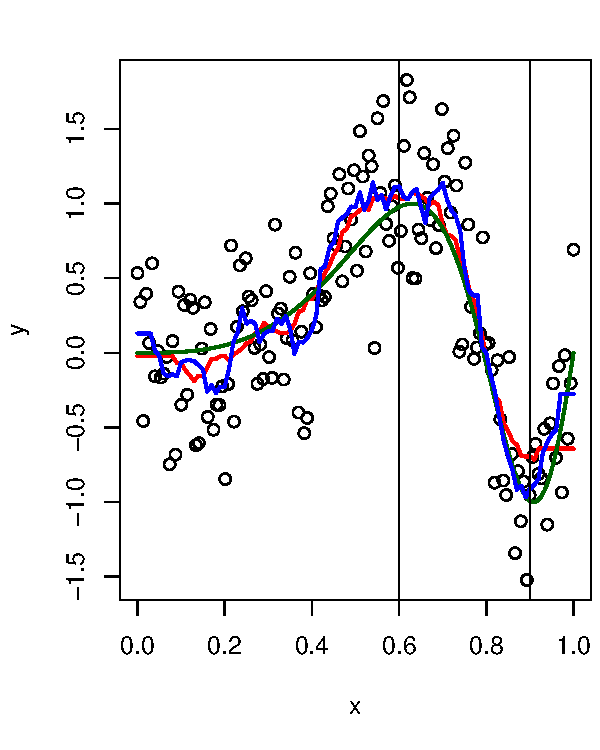
\includegraphics[width=0.95\textwidth]{figure/020-regression-1unnamed-chunk-10-1} 

\end{knitrout}
}%
\column{0.33\textwidth}
\onslide*<2-3>{
\begin{knitrout}
\definecolor{shadecolor}{rgb}{0.969, 0.969, 0.969}\color{fgcolor}
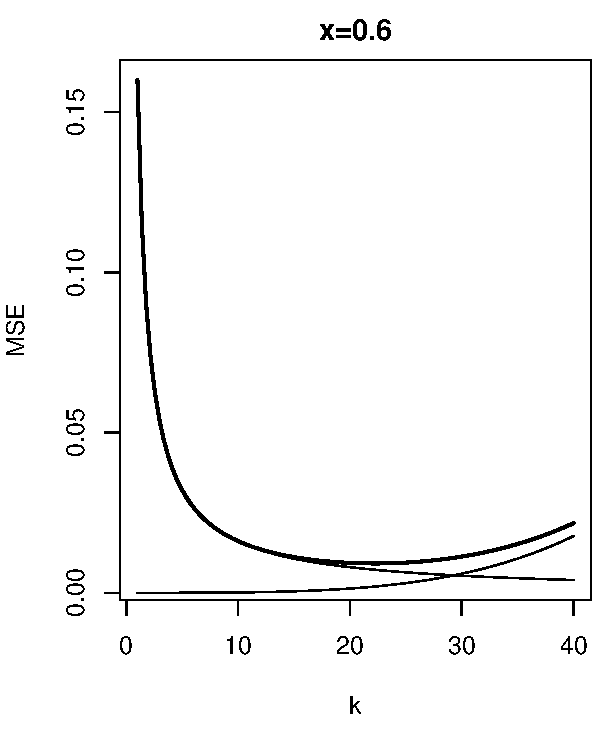
\includegraphics[width=0.95\textwidth]{figure/020-regression-1unnamed-chunk-11-1} 

\end{knitrout}
}%
\column{0.33\textwidth}
\onslide*<3>{
\begin{knitrout}
\definecolor{shadecolor}{rgb}{0.969, 0.969, 0.969}\color{fgcolor}
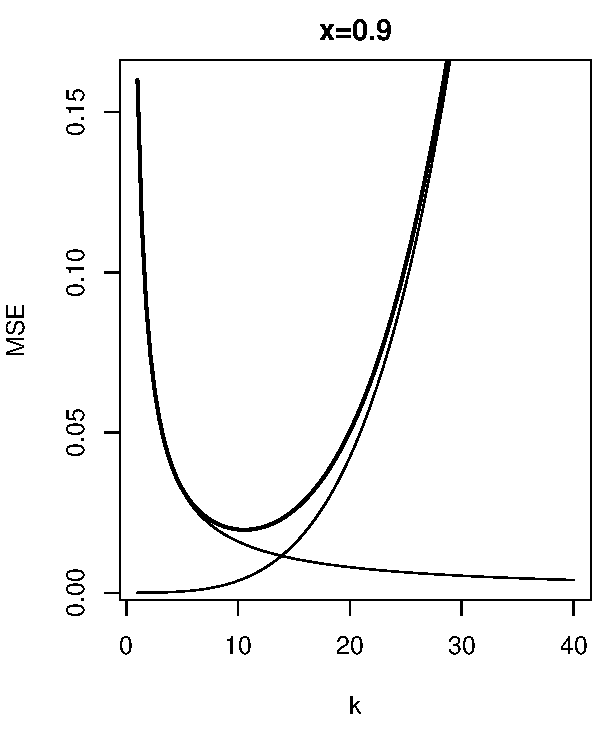
\includegraphics[width=0.95\textwidth]{figure/020-regression-1unnamed-chunk-12-1} 

\end{knitrout}
}%
\end{columns}

\end{frame}



\begin{frame}{Da $MSE(x)$ all'errore complessivo}
Disponiamo dell'MSE per $\hat{f}_k(x)$:
\[
 MSE(\hat{f}_k(x)) =  E((f(x)-\hat{f}_k(x))^2) = (f(x)-E(\hat{f}_k(x)))^2 + V(\hat{f}_k(x)) %= \mbox{bias}_x^2 + \mbox{variance}_x
\]
mettiamoli insieme per ottenere un errore complessivo
\[ R(k) = E\left(\frac{1}{n}\sum_{i=1}^n (\hat{f}_k(x_i) - f(x_i))^2\right) \]
%The MSE is usually estmated by the {\bf leave-one-out cross validation}
%\[
%CV = \hat{R}(h) =\frac{1}{n} \sum_{i=1}^n (Y_i - \hat{f}_{-i}(x_i))^2
%\]
%where $\hat{f}_i$ is the estimator obtained omitting the $i$-the pair $(x_i,Y_i)$.
\begin{columns}
\column{0.6\textwidth}
\begin{knitrout}
\definecolor{shadecolor}{rgb}{0.969, 0.969, 0.969}\color{fgcolor}
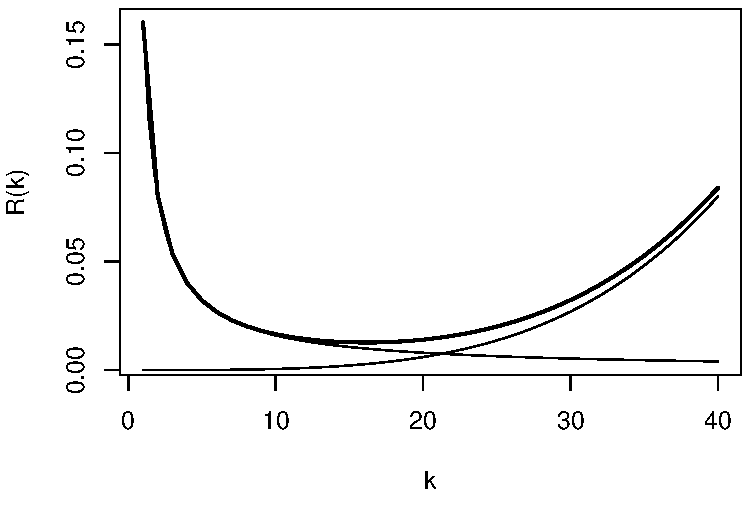
\includegraphics[width=0.9\textwidth]{figure/020-regression-1unnamed-chunk-13-1} 

\end{knitrout}
\column{0.4\textwidth}
La scelta di $k$ potrebbe basarsi su $R(k)$, ha senso scegliere $k=\mbox{argmin}_k R(k)$.
\end{columns}
\end{frame}

\begin{frame}{Stimatore di $R()$}
L'obiettivo \`e stimare
\[ R(k) = E\left(\frac{1}{n}\sum_{i=1}^n (\hat{f}_k(x_i) - f(x_i))^2\right) \]
(principalmente per individuare il valore ottimale di $k$.)

\spazio

Uno stimatore na\"if sarebbe
\[  \frac{1}{n} \sum_{i=1}^n (Y_i-\hat{f}_k(x_i))^2 \]
ma questo \`e ovviamente una sottostima in quanto ...

\end{frame}


\begin{frame}{Stimatore di $R()$: validazione incrociata uno  a uno}
Uno stimatore migliore per $R(k)$ \`e
\[
CV(k) = \hat{R}(k) =\frac{1}{n} \sum_{i=1}^n (Y_i - \hat{f}_{k,-i}(x_i))^2
\]
dove $\hat{f}_{k,-i}(x_i)$ \`e il lisciatore stimato {\bf senza} l'$i$-esima osservazione.

Si noti che
\begin{eqnarray*}
E(Y_i-\hat{f}_{k,-i}(x_i))^2 
&=& E(Y_i-f(x_i)+f(x_i)-\hat{f}_{k,-i}(x_i))^2 \\
&=& \sigma^2 + E(f(x_i)-\hat{f}_{h,-i}(x_i))^2 \\
&\approx& \sigma^2 + E(f(x_i)-\hat{f}_{k}(x_i))^2 
\end{eqnarray*}
Cio\`e, $\hat{R}$ \`e, approssimativamente, uno stimatore non distorto dell'errore di previsione
\[ E(\hat{R}) \approx R + \sigma^2  \]
\end{frame}


\begin{frame}{Lisciatori lineari}
Discutiamo della stima dell'errore per una classe di lisciatori che comprende quelli visti sopra e molti altri: i {\bf lisciatori lineari}, ovvero dei lisciatori per i quali esiste, per ogni $x$, un vettore $\ell(x)=(\ell_1(x),\ldots,\ell_n(x))^T$ tale che
\[ \hat{f}(x) = \sum_{i=1}^n \ell_i(x) Y_i  \]
il che significa che
\[
{\bf\hat{f}} =
\begin{bmatrix}
\hat{f}(x_1) \\ \vdots \\ \hat{f}(x_n)
\end{bmatrix}
=
\begin{bmatrix}
\ell_1(x_1) & \cdots & \ell_n(x_1) \\ \vdots \\ \ell_1(x_n) & \cdots & \ell_n(x_n) 
\end{bmatrix}
{\bf Y} 
= L{\bf Y}
\]
La matrice $L$ \`e la {\bf matrice di lisciamento}, si definiscono anche i gradi di libert\`a del lisciatore come
\[ \nu = tr(L) \]
\end{frame}

\begin{frame}{Lisciatori lineari}
I precedenti lisciatori sono tutti lisciatori lineari, ricaviamo le matrici $L$ ad essi associati. 
(Senza perdita di generalit\`a, si assume che le $x_i$ siano ordinate).
\begin{itemize}
\item regressogramma:  $L$ \`e diagonale a blocchi e assume valore pari al reciproco del numero di osservazioni in ciascun blocco.
\item medie mobili 
\begin{itemize}
\item vicini pi\`u vicini: $L$ \`e 0 ovunque tranne che su una striscia intorno alla diagonale dove vale $1/k$.
\item raggio: $L$ \`e analoga al caso precedente se le $x_i$ sono equidistanziate, altrimenti...
\end{itemize}
\end{itemize}
\end{frame}



\begin{frame}{Validazione incrociata uno  a uno per lisciatori lineari}
Per un lisciatore lineare definito dalla matrice $L$ 
\[
CV = \hat{R}(k) =\frac{1}{n} \sum_{i=1}^n (Y_i - \hat{f}_{k,-i}(x_i))^2
= \frac{1}{n} \sum_{i=1}^n\left(\frac{Y_i-\hat{f}_k(x_i)}{1-L_{ii}}\right)^2
\]
sicch\'e non necessita di ricalcolare il lisciatore ma solo di conoscere  $L_{ii}$.

\spazio

Un'ulteriore semplificazione \`e costituita dal {\bf criterio di validazione incrociata generalizzata} che prevede di sostituire $L_{ii}$ con il suo valore medio
\[ 
GCV = \frac{1}{n} \sum_{i=1}^n\left(\frac{Y_i-\hat{f}(x_i)}{1-\nu/n}\right)^2
\]
\end{frame}

\begin{frame}[allowframebreaks=0.95]{Derivazione delle formule per CV e GCV}
Definiamo $\hat{f}_{-i}(x_i)$. Essendo
\[
\hat{f}(x_i) = \sum_{j=1}^n \ell_j(x_i) y_j
\]
e assumendo $\sum_{j=1}^n \ell_j(x_i)=1$ (le costanti sono mantenute), definiamo
\[
\hat{f}_{-i}(x_i) = \frac{\sum_{j\neq i} \ell_j(x_i) y_j}{\sum_{j\neq i} \ell_j(x_i) } = \frac{\sum_{j\neq i} \ell_j(x_i) y_j}{1- \ell_i(x_i) }= \frac{\sum_{j\neq i} \ell_j(x_i) y_j}{1- L_{ii} }
\]

\spazio

Si noti che potremmo definire $\hat{f}_{-i}()$ come il lisciatore ri-stimato senza  $(x_i,y_i)$, la definizione \`e equivalente per lo stimatore a raggio, non per i $k$ pi\`u vicini.

\break

Con la formula sopra si ottiene
\begin{align*}
y_i-\hat{y}_{-i} 
&= y_i - \frac{1}{1-L_{ii}} \sum_{j\neq i} \ell_j(x_i) y_j \\
&= y_i - \frac{1}{1-L_{ii}} \left(\sum_{j=1}^n \ell_j(x_i) y_j - L_{ii}y_i\right) \\
&= y_i - \frac{1}{1-L_{ii}} \left(\hat{y}_i - L_{ii}y_i\right) \\
&= \frac{1}{1-L{ii}} \left((1-L_{ii})y_i - \hat{y}_i + L_{ii}y_i\right) = \frac{1}{1-L{ii}}(y_i-\hat{y}_i) 
\end{align*}
e quindi la formula del GCV.


\end{frame}


\begin{frame}{Altri criteri}
Si noti che, essendo $(1-x)^{-2}\approx 1+2x$ in un intorno di $0$, il GCV \`e approssimativamente uguale al $C_p$ di Mallow.
\[ 
GCV = \frac{1}{n} \sum_{i=1}^n\left(\frac{Y_i-\hat{f}(x_i)}{1-\nu/n}\right)^2
\approx \frac{1}{n} \sum_{i=1}^n\left(Y_i-\hat{f}(x_i)\right)^2 + \frac{2\nu\hat{\sigma}^2}{n} = C_p
\]
Pi\`u in generale, molti criteri usati per la scelta del grado di lisciamento ($k$) hanno la forma
\[
B(k) = \Lambda(n,k)\frac{1}{n} + \sum_{i=1}^n\left(Y_i-\hat{f}(x_i)\right)^2 
\]
per qualche funzione $\Lambda(\cdot,\cdot)$
\end{frame}

\section[Nucleo]{Regressione col metodo del nucleo}

\begin{frame}{Kernel regression}
Con i metodi descritti sin qui, man mano che ci si muove lungo l-asse $x$, si calcola $\hat{f}(x)$ come media di differenti gruppi di osservazioni $y_i$.

\spazio

Questo porta a una stima finale poco ``liscia''.

\spazio

Un modo di lisciare maggiormente \`e di usare una media pesata dove il peso delle osservazioni decresce man mano che ci si allontana da $x$.
\end{frame}

\begin{frame}{Stimatore di Nadaraya-Watson}
Lo stimatore di Nadaraya-Watson \`e  un lisciatore lineare
\[ \hat{f}(x) = \sum_{i=1}^n \ell_i(x) Y_i  \]
in cui
\[ \ell_i(x) = \frac{K\left(\frac{x-x_i}{h}\right)}{\sum_{j=1}^n K\left(\frac{x-x_j}{h}\right)} \]
dove $K()$ \`e un nucleo.
\end{frame}

\begin{frame}{Nuclei}
\begin{columns}
\column{0.5\textwidth}
Si ha
%\begin{tiny}
\[
\hat{f}_n(x) = \frac{\sum_{i=1}^n K\left(\frac{x-X_i}{h}\right)Y_i}{\sum_{i=1}^n K\left(\frac{x-X_i}{h}\right)} 
\]
%\end{tiny}
dove $K$ \`e tale che
\begin{itemize}
\item $ K(x)\geq 0$
\item $ \int K(x)dx=1$
\item $ \int xK(x)dx=0$
\item $ \int x^2K(x)dx>0$
\end{itemize}
\column{0.5\textwidth}
Esempi di nuclei

\begin{tabular}{cc}\hline
& $K(u)$ \\\hline
Uniform & $\frac{1}{2}I_{[-1,1]}(u)$ \\
Triangle & $(1-|u|)I_{[-1,1]}(u)$ \\
Triweight & $\frac{35}{32}(1-u^2)^3I_{[-1,1]}(u)$ \\
Quartic & $\frac{15}{16}(1-u^2)^2I_{[-1,1]}(u)$ \\
Gaussian & $\frac{1}{\sqrt{2\pi}} e^{-u^2/2}$ \\
Epanechnikov & $\frac{3}{4}(1-u^2)I_{[-1,1]}(u)$ \\
Cosine & $\frac{\pi}{4}\cos\left(\frac{\pi}{2}u\right)I_{[-1,1]}(u)$ \\\hline
\end{tabular}
\end{columns}
\end{frame}






\begin{frame}{Kernel functions}

\begin{tabular}{cccc}
Uniform &
\multirow{4}{*}{
\includegraphics[width=0.05\textwidth]{figure/Uniform} 
}%
& 
Triangle &
\multirow{4}{*}{
\includegraphics[width=0.05\textwidth]{figure/Triangle} 
}%
\\
$\frac{1}{2}I_{[-1,1]}(u)$ & &  $(1-|u|)I_{[-1,1]}(u)$ & \\ & & & \\ & & & \\
Triweight &
\multirow{4}{*}{
\includegraphics[width=0.05\textwidth]{figure/Triweight} 
}%
& 
Quartic &
\multirow{4}{*}{
\includegraphics[width=0.05\textwidth]{figure/Quartic} 
}%
\\
 $\frac{35}{32}(1-u^2)^3I_{[-1,1]}(u)$ & &   $\frac{15}{16}(1-u^2)^2I_{[-1,1]}(u)$ & \\ & & & \\ & & & \\
Cosine &
\multirow{4}{*}{
\includegraphics[width=0.05\textwidth]{figure/Cosine} 
}%
& 
Epanechnikov &
\multirow{4}{*}{
\includegraphics[width=0.05\textwidth]{figure/Epanechnikov} 
}%
\\
$\frac{\pi}{4}\cos\left(\frac{\pi}{2}u\right)I_{[-1,1]}(u)$ & &    $\frac{3}{4}(1-u^2)I_{[-1,1]}(u)$  & \\ & & & \\ & & & \\
Gaussian &
\multirow{4}{*}{
\includegraphics[width=0.05\textwidth]{figure/Gaussian} 
}%
& 
 &
\multirow{4}{*}{}%
\\
$\frac{1}{\sqrt{2\pi}} e^{-u^2/2}$ & &      & \\ & & & \\ & & & \\

\end{tabular}
\end{frame}


\begin{frame}{Nadaraya-Watson estimator: risk}
Si mostra che, se $x_i$ proviene dalla densit\`a $g()$, per $h_n\rightarrow 0$ e $nh_n\rightarrow\infty$
\begin{align*}
R = &\frac{h_n^4}{4}\left(\int u^2K(u)du\right)^2\int \left(f''(x)+2f'(x)\frac{g'(x)}{g(x)}\right)^2dx \\
&\phantom{====}+ \frac{\sigma^2\int K^2(u)du}{nh_n}\int\frac{1}{g(x)}dx +o(nh_n^{-1}) +o(h_n^4)
\end{align*}

Dove si nota che
\begin{itemize}
\item la varianza decresce con $h$
\item la distorsione cresce con $h^4$
\item la distorsione cresce con  $f''$
\item la distorsione cresce con  $f'(x)\frac{g'(x)}{g(x)}$: {\it design bias}
\end{itemize}
\end{frame}


\begin{frame}{Design bias e boundary bias}
\begin{knitrout}
\definecolor{shadecolor}{rgb}{0.969, 0.969, 0.969}\color{fgcolor}
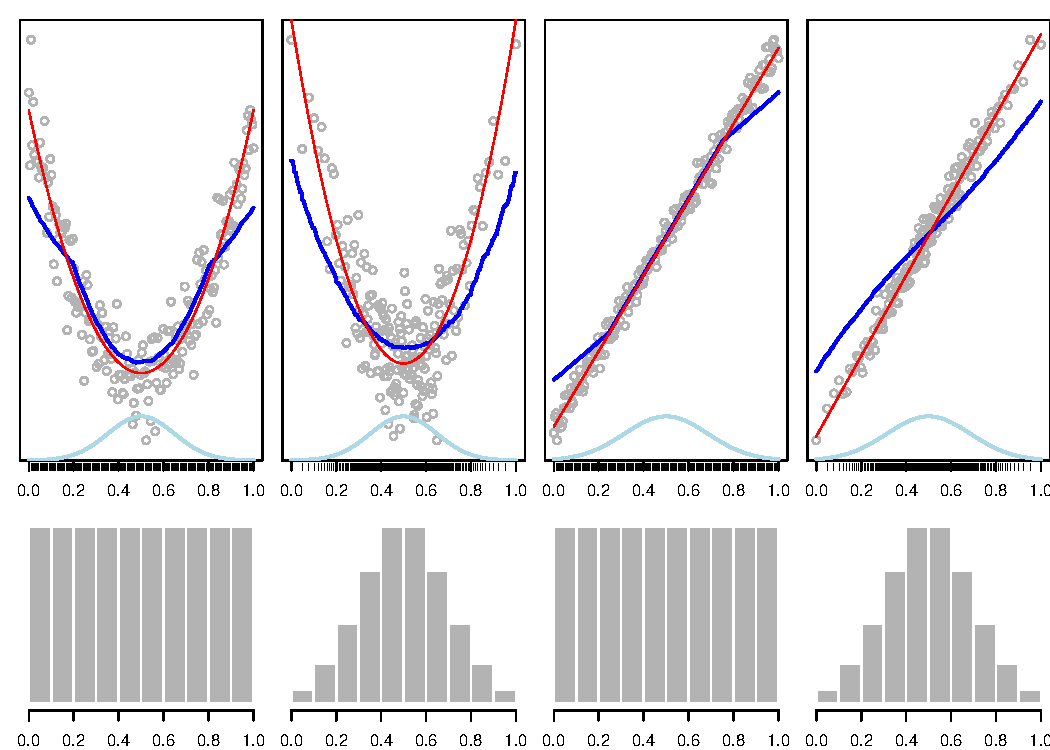
\includegraphics[width=0.9\textwidth]{figure/020-regression-1unnamed-chunk-14-1} 

\end{knitrout}
\end{frame}



\begin{frame}{Boundary bias}
\begin{knitrout}
\definecolor{shadecolor}{rgb}{0.969, 0.969, 0.969}\color{fgcolor}
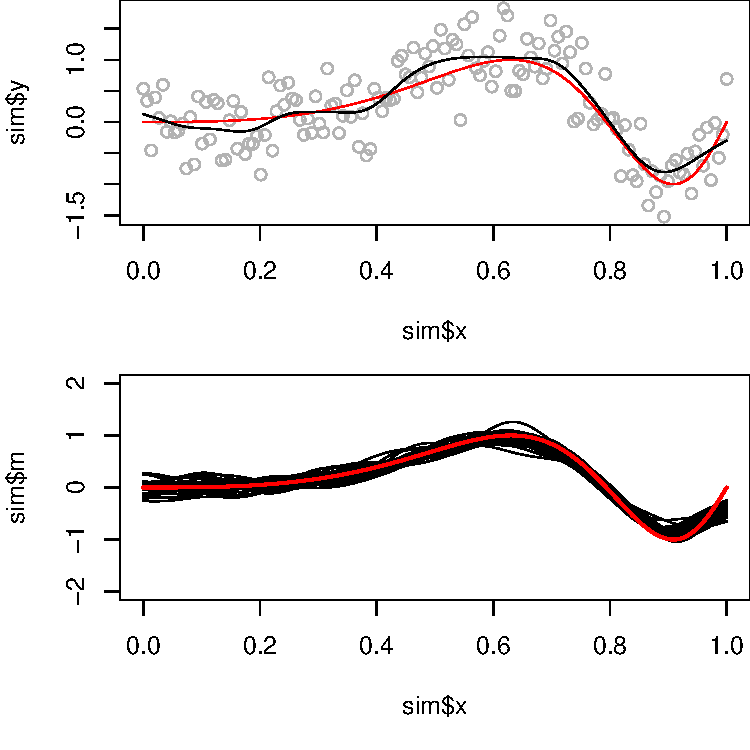
\includegraphics[width=0.7\textwidth]{figure/020-regression-1unnamed-chunk-15-1} 

\end{knitrout}
\end{frame}


\begin{frame}{N-W come mimimo \onslide*<2->{$\rightarrow$ polinomi locali}}
\onslide*<1>{
Notiamo che lo stimatore di N-W in $x$, $\hat{f}(x)$, \`e la soluzione di
\[ \underset{a}{\mbox{argmin}} \sum_{i=1}^n K_i\left(\frac{x_i-x}{h}\right)(Y_i - a)^2 \]
cio\`e, lo stimatore di N-W \`e, localmente, uno stimatore dei minimi quadrati pesati.

\spazio
}
\onslide*<1->{
Si potrebbe allora impiegare i minimi quadrati pesati ma con un polinomio anzich\`e una costante, per ogni valore di $x$ si approssima  $f()$ in un intorno di $x$ con il polinomio
\[ p_x(u;{\bf a}) = a_0 + a_1(u-x) + \frac{a_2}{2!}(u-x)^2 +\ldots + \frac{a_p}{p!}(u-x)^p \]
}
\onslide*<2->{
e si stima ${\bf a}(x)$ (rendiamo esplicita la dipendenza da $x$) minimizzando
\[ \hat{\bf a}(x) = \underset{a}{\mbox{argmin}} \sum_{i=1}^n K_i\left(\frac{x_i-x}{h}\right)(Y_i - p_x(X_i;{\bf a}))^2 \]
e definiamo il seguente stimatore di $f(x)$ 
\[ \hat{f}(x) = p_x(x,\hat{\bf a}) = \hat{a}_0(x) \]
}
\end{frame}

\begin{frame}{Polinomi locali, notazione matriciale}
\onslide*<1>{
Sia
\[
X_x=
\begin{bmatrix}
1 & x_1-x & \cdots & \frac{1}{p!}(x_1-x)^p \\
\vdots & \vdots & & \vdots\\
1 & x_n-x & \cdots & \frac{1}{p!}(x_n-x)^p \\
\end{bmatrix}
\]
\[
W_x =\mbox{diag}\left\{K_i\left(\frac{x_i-x}{h}\right), i=1,\ldots, n\right\}
\]
allora la somma dei quadrati pesata \`e
\[
({\bf Y} -X_x{\bf a})^T W_x ({\bf Y} -X_x{\bf a})
\]
e
}
\onslide*<1->{
\[
\hat{\bf a} = (X_x^TW_xX_x)^TX_x^TW_x{\bf Y}
\]
}
\onslide*<2->{
Lo stimatore $\hat{f}(x)=\hat{a}_0(x)$ \`e dunque
\[ 
\hat{f}(x) = e_1^T(X_x^TW_xX_x)^TX_x^TW_x{\bf Y}
\]
dove $e_1^T=(1,0,\ldots,0)$.

Quindi $\hat{f}(x)$ \`e un lisciatore lineare
\[ \hat{f}(x) = \sum_{i=1}^n \ell_i(x) Y_i \]
dove
\[ \ell(x)^T = (\ell_1(x),\ldots,\ell_n(x))^T = e_1^T(X_x^TW_xX_x)^TX_x^TW_x \]
}
\end{frame}

\begin{frame}{Lisciatore lineare locale}
Posto $p=1$, si ottiene lo stimatore lineare locale
\[ \ell_i(x) = \frac{b_i(x)}{\sum_{j=1}^n b_j(x)} \]
dove
\[ b_i(x) = K\left(\frac{x_i-x}{h}\right)(S_{n,2}(x)-(x_i-x)S_{n,1}(x)) \]
\[ S_{n,j}(x) = \sum_{i=1}^nK\left(\frac{x_i-x}{h}\right)(x_i-x)^j,\;\;j=1,2\]
\end{frame}

\begin{frame}{Lisciatore lineare locale: distorsione e varianza}
Si mostra che il rischio in $x$ \`e
\begin{eqnarray*}
R_x = \frac{h_n^4}{4}\left( \int u^2K(u)du\right)^2 f''(x)^2 + \frac{\sigma^2\int K^2(u)du}{g(x)nh_n} +o(nh_n^{-1}) +o(h_n^4)
\end{eqnarray*}
\onslide<2>{
Se lo confrontiamo con quello dello stimatore di N-W notiamo che \`e scomparso il {\it design bias}.
\begin{align*}
R = &\frac{h_n^4}{4}\left(\int u^2K(u)du\right)^2\int \left(f''(x)+2f'(x)\frac{g'(x)}{g(x)}\right)^2dx \\
&\phantom{====}+ \frac{\sigma^2\int K^2(u)du}{nh_n}\int\frac{1}{g(x)}dx +o(nh_n^{-1}) +o(h_n^4)
\end{align*}

}

\end{frame}



\begin{frame}{Graphical representation}
\begin{knitrout}
\definecolor{shadecolor}{rgb}{0.969, 0.969, 0.969}\color{fgcolor}



































































































\animategraphics[width=0.9\textwidth,height=0.8\textheight,controls,loop]{1}{figure/020-regression-1animazregloc-}{1}{100}

\end{knitrout}
\end{frame}

\begin{frame}{Graphical representation}
\begin{knitrout}
\definecolor{shadecolor}{rgb}{0.969, 0.969, 0.969}\color{fgcolor}



































































































\animategraphics[width=0.9\textwidth,height=0.8\textheight,controls,loop]{1}{figure/020-regression-1animazreglochbasso-}{1}{100}

\end{knitrout}
\end{frame}

\begin{frame}{Graphical representation: comparison}
\begin{knitrout}
\definecolor{shadecolor}{rgb}{0.969, 0.969, 0.969}\color{fgcolor}



































































































\animategraphics[width=0.9\textwidth,height=0.8\textheight,controls,loop]{1}{figure/020-regression-1animazreglochdoppia-}{1}{100}

\end{knitrout}
\end{frame}




\begin{frame}{Boundary bias}

N-W versus local linear, same bandwith
\begin{center}
\begin{knitrout}
\definecolor{shadecolor}{rgb}{0.969, 0.969, 0.969}\color{fgcolor}
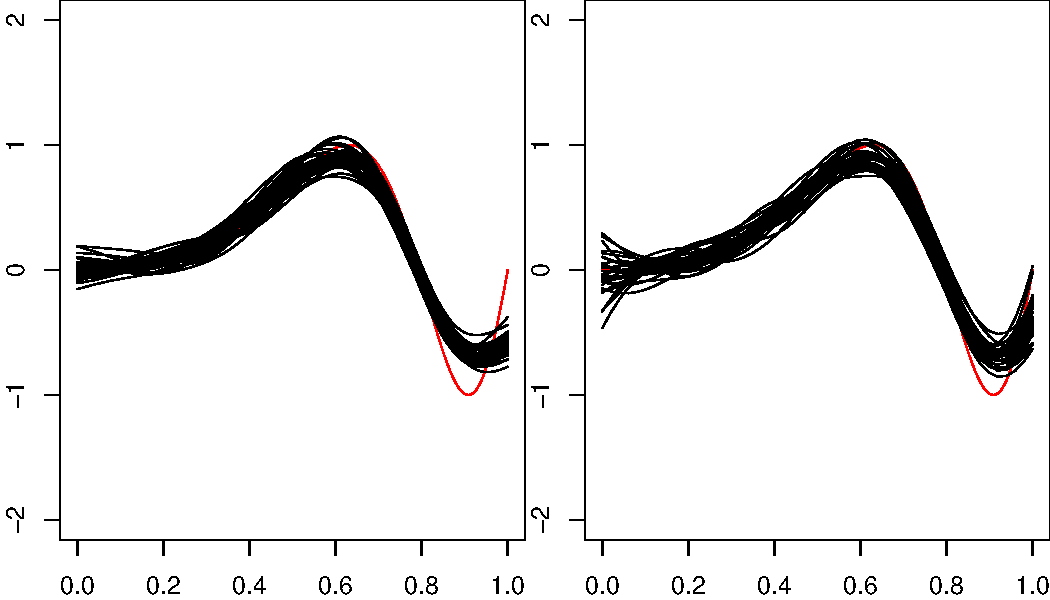
\includegraphics[width=0.7\textwidth]{figure/020-regression-1unnamed-chunk-16-1} 

\end{knitrout}
\end{center}

\end{frame}


\begin{frame}{Design bias and boundary bias}
\begin{knitrout}
\definecolor{shadecolor}{rgb}{0.969, 0.969, 0.969}\color{fgcolor}
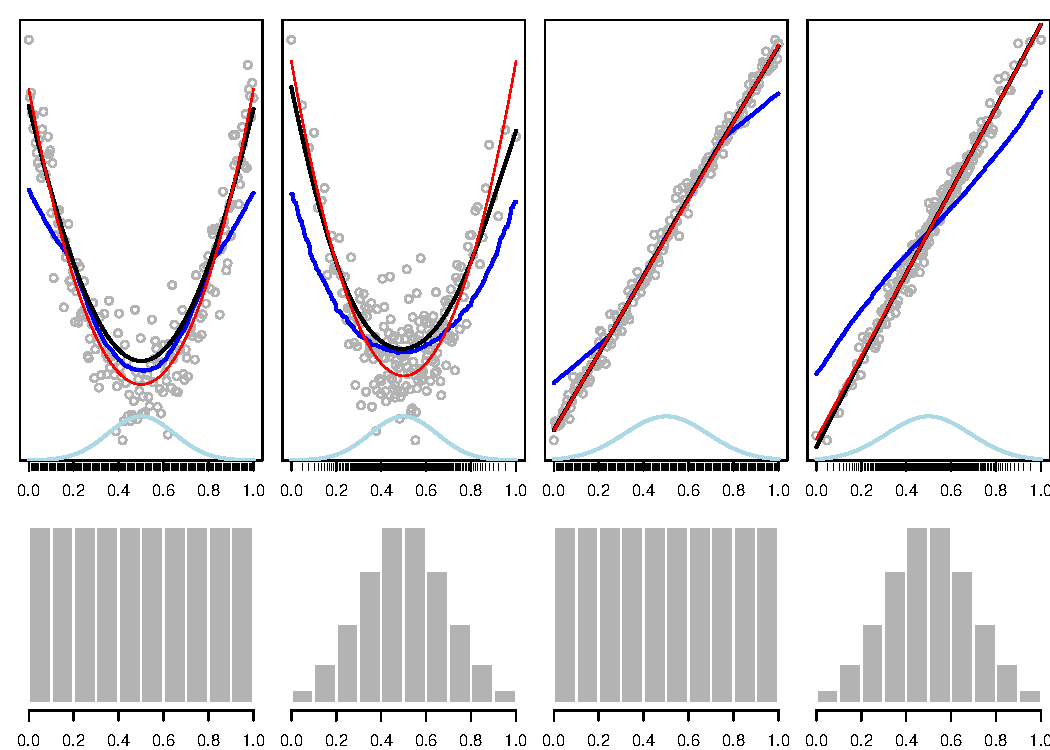
\includegraphics[width=0.9\textwidth]{figure/020-regression-1unnamed-chunk-17-1} 

\end{knitrout}
\end{frame}




\begin{knitrout}
\definecolor{shadecolor}{rgb}{0.969, 0.969, 0.969}\color{fgcolor}\begin{kframe}


{\ttfamily\noindent\bfseries\color{errorcolor}{Error in eval(expr, envir, enclos): oggetto "{}lidar"{} non trovato}}\end{kframe}
\end{knitrout}

\begin{frame}[fragile]{LIDAR: modello polinomiale}
Assumiamo che $f()$ sia (approssimabile da) un polinomio
\[ f(x;\vbeta) = \beta_0 + \beta_1 x + \beta_2 x^2 + \ldots + \beta_{p} x^p \]
\begin{columns}[T]
\column{0.5\textwidth}
\begin{knitrout}
\definecolor{shadecolor}{rgb}{0.969, 0.969, 0.969}\color{fgcolor}\begin{kframe}


{\ttfamily\noindent\bfseries\color{errorcolor}{Error in eval(expr, envir, enclos): oggetto "{}lidar"{} non trovato}}

{\ttfamily\noindent\bfseries\color{errorcolor}{Error in eval(expr, envir, enclos): oggetto "{}lidar"{} non trovato}}

{\ttfamily\noindent\bfseries\color{errorcolor}{Error in plot(lidar\$range, lidar\$logratio, pch = 20, xlab = "{}range (standardized)"{}, : oggetto "{}lidar"{} non trovato}}

{\ttfamily\noindent\bfseries\color{errorcolor}{Error in plot.xy(xy.coords(x, y), type = type, ...): plot.new has not been called yet}}

{\ttfamily\noindent\bfseries\color{errorcolor}{Error in plot.xy(xy.coords(x, y), type = type, ...): plot.new has not been called yet}}

{\ttfamily\noindent\bfseries\color{errorcolor}{Error in strwidth(legend, units = "{}user"{}, cex = cex, font = text.font): plot.new has not been called yet}}\end{kframe}
\end{knitrout}
\column{0.5\textwidth}
Il ruolo di $k$ \`e svolto da $p$, al crescere di $p$
\begin{itemize}
\item aumenta la varianza
\item diminuisce la distorsione
\end{itemize}
Problema: elevata correlazione dei $\hat\beta_j$
\begin{scriptsize}
% latex table generated in R 3.5.3 by xtable 1.8-4 package
% Wed Jul 17 16:28:59 2019
\begin{tabular}{rrrrr}
  \hline
 & x & I(x\verb|^|2) & I(x\verb|^|3) & I(x\verb|^|4) \\ 
  \hline
x & 1.00 & -0.97 & 0.92 & -0.86 \\ 
  I(x\verb|^|2) & -0.97 & 1.00 & -0.99 & 0.95 \\ 
  I(x\verb|^|3) & 0.92 & -0.99 & 1.00 & -0.99 \\ 
  I(x\verb|^|4) & -0.86 & 0.95 & -0.99 & 1.00 \\ 
   \hline
\end{tabular}

\end{scriptsize}
\end{columns}

\end{frame}


\begin{frame}[fragile]{LIDAR: modello lineare a tratti}
In alternativa, si potrebbe usare un modello lineare a tratti
\[ f(x;\vbeta) = \beta_{0,j} + \beta_{1,j} x \mbox{ se } c_{j-1}\leq x < c_j,\;j=1,\ldots,J \]
avendo suddiviso il supporto di $x$ in intervalli (cfr costante a tratti).
\begin{columns}[T]
\column{0.5\textwidth}
\begin{knitrout}
\definecolor{shadecolor}{rgb}{0.969, 0.969, 0.969}\color{fgcolor}\begin{kframe}


{\ttfamily\noindent\bfseries\color{errorcolor}{Error in eval(expr, envir, enclos): oggetto "{}lidar"{} non trovato}}

{\ttfamily\noindent\bfseries\color{errorcolor}{Error in eval(expr, envir, enclos): oggetto "{}lidar"{} non trovato}}

{\ttfamily\noindent\bfseries\color{errorcolor}{Error in plot(lidar\$range, lidar\$logratio, pch = 20, xlab = "{}range (standardized)"{}, : oggetto "{}lidar"{} non trovato}}

{\ttfamily\noindent\bfseries\color{errorcolor}{Error in plot.xy(xy.coords(x, y), type = type, ...): plot.new has not been called yet}}\end{kframe}
\end{knitrout}
\column{0.5\textwidth}
Il ruolo di $k$ \`e svolto da $J$, al crescere di $J$
\begin{itemize}
\item aumenta la varianza
\item diminuisce la distorsione
\end{itemize}
Problema: la funzione che si ottiene non \`e continua.
\end{columns}

\end{frame}



\section{Spline}


\begin{frame}{Spline lineare: esempio con due nodi}
\onslide*<1>{
Una soluzione pi\`u sofisticata si ottiene con
\[ y_i = \beta_1+\beta_2 x_i + \beta_3 (x_i-\nu_1)_+ + \beta_4 (x_i-\nu_2)_+ +\varepsilon_i \]
dove
\[
(x)_+=\begin{cases} x &\mbox{se }x>0 \\ 0 &\mbox{altrimenti}\end{cases};
\;\;\;\;
(x-\nu)_+=\begin{cases} x-\nu &\mbox{se }x>\nu \\ 0 &\mbox{altrimenti}\end{cases}
\]
\begin{itemize}
\item $\varepsilon_i \thicksim IID(\mathcal N(0,\sigma^2))$, 
\item $\nu_1$ e $\nu_2$, detti nodi, sono valori fissati nel supporto di $x$
\item $\beta_i$ sono stimati come al solito:
\[ \hat{\vbeta} = \underset{\vbeta}{\text{argmin}} \sum_{i=1}^n (y_i-f(x_i;\vbeta))^2 \]
dove
\[ f(x_i;\vbeta) = \beta_1+\beta_2 x_i + \beta_3 (x_i-\nu_1)_+ + \beta_4 (x_i-\nu_2)_+ \]
\end{itemize}
}

\onslide*<2>{
\begin{columns}
\column{0.6\textwidth}

\begin{knitrout}
\definecolor{shadecolor}{rgb}{0.969, 0.969, 0.969}\color{fgcolor}\begin{kframe}


{\ttfamily\noindent\bfseries\color{errorcolor}{Error in plot(lidar\$range, lidar\$logratio, pch = 20, xlab = "{}range (standardized)"{}, : oggetto "{}lidar"{} non trovato}}

{\ttfamily\noindent\bfseries\color{errorcolor}{Error in eval(expr, envir, enclos): oggetto "{}lidar"{} non trovato}}

{\ttfamily\noindent\bfseries\color{errorcolor}{Error in cbind(lidar1, fbase(lidar1\$range, i, p)): oggetto "{}lidar1"{} non trovato}}

{\ttfamily\noindent\bfseries\color{errorcolor}{Error in is.data.frame(data): oggetto "{}lidar1"{} non trovato}}

{\ttfamily\noindent\bfseries\color{errorcolor}{Error in lines(lidar\$range, predict(fit), col = "{}red"{}, lwd = 2): oggetto "{}lidar"{} non trovato}}

{\ttfamily\noindent\bfseries\color{errorcolor}{Error in axis(side = side, at = at, labels = labels, ...): plot.new has not been called yet}}\end{kframe}
\end{knitrout}

\begin{knitrout}
\definecolor{shadecolor}{rgb}{0.969, 0.969, 0.969}\color{fgcolor}\begin{kframe}


{\ttfamily\noindent\bfseries\color{errorcolor}{Error in eval(expr, envir, enclos): oggetto "{}lidar"{} non trovato}}

{\ttfamily\noindent\bfseries\color{errorcolor}{Error in curve(fbase1(x, nodi[length(nodi)], p), xlim = range(lidar\$range), : oggetto "{}lidar"{} non trovato}}\end{kframe}
\end{knitrout}

\column{0.4\textwidth}
\`E un modello lineare con esplicative
\[ x_i,\;(x_i-\nu_1)_+,\;(x_i-\nu_2)_+ \]
La funzione $\hat{f}(x)$ \`e una combinazione lineare delle funzioni 
\begin{align*}
B_0(x) &=x\\ 
B_1(x) &=(x-\nu_1)_+\\
B_2(x) &=(x-\nu_2)_+ 
\end{align*}
dette funzioni base (in blu nel grafico).
\end{columns}
}
\end{frame}


\begin{frame}{Spline lineare: $K$ nodi}
\onslide*<1>{
Pi\`u in generale, si fissano $K$ nodi
\[ \nu_1,\ldots, \nu_K \]
e si stima il modello lineare (attenzione alla notazione!)
\[ y_i = \beta_1+\beta_2 x_i + \sum_{k=1}^K b_k (x_i-\nu_k)_+ + \varepsilon_i \]
La funzione spline \`e rappresentata da
\[ f(x) = \beta_1+\beta_2 x + \sum_{k=1}^K b_k (x-\nu_k)_+ \]
ed \`e tanto pi\`u liscia quanti meno nodi si usano (minore $K$).
}
\onslide*<2>{
\begin{knitrout}
\definecolor{shadecolor}{rgb}{0.969, 0.969, 0.969}\color{fgcolor}\begin{kframe}


{\ttfamily\noindent\bfseries\color{errorcolor}{Error in seq(min(lidar\$range), max(lidar\$range), by = 0.25): oggetto "{}lidar"{} non trovato}}\end{kframe}
\end{knitrout}
\begin{knitrout}
\definecolor{shadecolor}{rgb}{0.969, 0.969, 0.969}\color{fgcolor}\begin{kframe}


{\ttfamily\noindent\bfseries\color{errorcolor}{Error in plot(lidar\$range, lidar\$logratio, pch = 20, xlab = "{}range (standardized)"{}, : oggetto "{}lidar"{} non trovato}}

{\ttfamily\noindent\bfseries\color{errorcolor}{Error in eval(expr, envir, enclos): oggetto "{}lidar"{} non trovato}}

{\ttfamily\noindent\bfseries\color{errorcolor}{Error in cbind(lidar1, fbase(lidar1\$range, i, p)): oggetto "{}lidar1"{} non trovato}}

{\ttfamily\noindent\bfseries\color{errorcolor}{Error in is.data.frame(data): oggetto "{}lidar1"{} non trovato}}

{\ttfamily\noindent\bfseries\color{errorcolor}{Error in lines(lidar\$range, predict(fit), col = "{}red"{}, lwd = 2): oggetto "{}lidar"{} non trovato}}

{\ttfamily\noindent\bfseries\color{errorcolor}{Error in axis(side = side, at = at, labels = labels, ...): plot.new has not been called yet}}\end{kframe}
\end{knitrout}

\begin{knitrout}
\definecolor{shadecolor}{rgb}{0.969, 0.969, 0.969}\color{fgcolor}\begin{kframe}


{\ttfamily\noindent\bfseries\color{errorcolor}{Error in eval(expr, envir, enclos): oggetto "{}lidar"{} non trovato}}

{\ttfamily\noindent\bfseries\color{errorcolor}{Error in curve(fbase1(x, nodi[length(nodi)], p), xlim = range(lidar\$range), : oggetto "{}lidar"{} non trovato}}\end{kframe}
\end{knitrout}
}
\onslide*<3>{

\begin{knitrout}
\definecolor{shadecolor}{rgb}{0.969, 0.969, 0.969}\color{fgcolor}\begin{kframe}


{\ttfamily\noindent\bfseries\color{errorcolor}{Error in plot(lidar\$range, lidar\$logratio, pch = 20, xlab = "{}range (standardized)"{}, : oggetto "{}lidar"{} non trovato}}

{\ttfamily\noindent\bfseries\color{errorcolor}{Error in eval(expr, envir, enclos): oggetto "{}lidar"{} non trovato}}

{\ttfamily\noindent\bfseries\color{errorcolor}{Error in cbind(lidar1, fbase(lidar1\$range, i, p)): oggetto "{}lidar1"{} non trovato}}

{\ttfamily\noindent\bfseries\color{errorcolor}{Error in is.data.frame(data): oggetto "{}lidar1"{} non trovato}}

{\ttfamily\noindent\bfseries\color{errorcolor}{Error in lines(lidar\$range, predict(fit), col = "{}red"{}, lwd = 2): oggetto "{}lidar"{} non trovato}}

{\ttfamily\noindent\color{warningcolor}{Warning in rug(nodi, lwd = 4, col = "{}blue"{}): some values will be clipped}}

{\ttfamily\noindent\bfseries\color{errorcolor}{Error in axis(side = side, at = at, labels = labels, ...): plot.new has not been called yet}}\end{kframe}
\end{knitrout}

\begin{knitrout}
\definecolor{shadecolor}{rgb}{0.969, 0.969, 0.969}\color{fgcolor}\begin{kframe}


{\ttfamily\noindent\bfseries\color{errorcolor}{Error in eval(expr, envir, enclos): oggetto "{}lidar"{} non trovato}}

{\ttfamily\noindent\bfseries\color{errorcolor}{Error in curve(fbase1(x, nodi[length(nodi)], p), xlim = range(lidar\$range), : oggetto "{}lidar"{} non trovato}}\end{kframe}
\end{knitrout}
}
\end{frame}




\begin{frame}{Base con potenze troncate}
\onslide*<1>{
Una naturale estensione della base lineare \`e data dalle potenze
\[ y_i = \beta_1+\beta_2 x_i + \ldots + \beta_{p+1}x^p + \sum_{k=1}^K b_k (x_i-\nu_k)_+^p + \varepsilon_i \]
sicch\'e la spline di ordine $p$ con $K$ nodi \`e
\[ f(x) = \beta_1+\beta_2 x + \ldots + \beta_{p+1}x^p + \sum_{k=1}^K b_k (x-\nu_k)_+^p \]
\begin{itemize}
\item Una spline di grado $p$ ha $p-1$ derivate continue, 
\item $p=3$ \`e adeguato per gli scopi usuali.
\end{itemize}
}
\onslide*<2>{

\begin{knitrout}
\definecolor{shadecolor}{rgb}{0.969, 0.969, 0.969}\color{fgcolor}\begin{kframe}


{\ttfamily\noindent\bfseries\color{errorcolor}{Error in plot(lidar\$range, lidar\$logratio, pch = 20, xlab = "{}range (standardized)"{}, : oggetto "{}lidar"{} non trovato}}

{\ttfamily\noindent\bfseries\color{errorcolor}{Error in eval(expr, envir, enclos): oggetto "{}lidar"{} non trovato}}

{\ttfamily\noindent\bfseries\color{errorcolor}{Error in cbind(lidar1, fbase(lidar1\$range, i, p)): oggetto "{}lidar1"{} non trovato}}

{\ttfamily\noindent\bfseries\color{errorcolor}{Error in is.data.frame(data): oggetto "{}lidar1"{} non trovato}}

{\ttfamily\noindent\bfseries\color{errorcolor}{Error in lines(lidar\$range, predict(fit), col = "{}red"{}, lwd = 2): oggetto "{}lidar"{} non trovato}}

{\ttfamily\noindent\color{warningcolor}{Warning in rug(nodi, lwd = 4, col = "{}blue"{}): some values will be clipped}}

{\ttfamily\noindent\bfseries\color{errorcolor}{Error in axis(side = side, at = at, labels = labels, ...): plot.new has not been called yet}}\end{kframe}
\end{knitrout}

\begin{knitrout}
\definecolor{shadecolor}{rgb}{0.969, 0.969, 0.969}\color{fgcolor}\begin{kframe}


{\ttfamily\noindent\bfseries\color{errorcolor}{Error in curve(fbase1(x, i, p), add = FALSE, lwd = 2, col = "{}blue"{}, xlim = range(lidar\$range), : oggetto "{}lidar"{} non trovato}}

{\ttfamily\noindent\bfseries\color{errorcolor}{Error in curve(fbase1(x, nodi[length(nodi)], p), xlim = range(lidar\$range), : oggetto "{}lidar"{} non trovato}}\end{kframe}
\end{knitrout}
}
\onslide*<3>{
\begin{knitrout}
\definecolor{shadecolor}{rgb}{0.969, 0.969, 0.969}\color{fgcolor}\begin{kframe}


{\ttfamily\noindent\bfseries\color{errorcolor}{Error in seq(min(lidar\$range), max(lidar\$range), by = 0.25): oggetto "{}lidar"{} non trovato}}\end{kframe}
\end{knitrout}
\begin{knitrout}
\definecolor{shadecolor}{rgb}{0.969, 0.969, 0.969}\color{fgcolor}\begin{kframe}


{\ttfamily\noindent\bfseries\color{errorcolor}{Error in plot(lidar\$range, lidar\$logratio, pch = 20, xlab = "{}range (standardized)"{}, : oggetto "{}lidar"{} non trovato}}

{\ttfamily\noindent\bfseries\color{errorcolor}{Error in eval(expr, envir, enclos): oggetto "{}lidar"{} non trovato}}

{\ttfamily\noindent\bfseries\color{errorcolor}{Error in cbind(lidar1, fbase(lidar1\$range, i, p)): oggetto "{}lidar1"{} non trovato}}

{\ttfamily\noindent\bfseries\color{errorcolor}{Error in is.data.frame(data): oggetto "{}lidar1"{} non trovato}}

{\ttfamily\noindent\bfseries\color{errorcolor}{Error in lines(lidar\$range, predict(fit), col = "{}red"{}, lwd = 2): oggetto "{}lidar"{} non trovato}}

{\ttfamily\noindent\color{warningcolor}{Warning in rug(nodi, lwd = 4, col = "{}blue"{}): some values will be clipped}}

{\ttfamily\noindent\bfseries\color{errorcolor}{Error in axis(side = side, at = at, labels = labels, ...): plot.new has not been called yet}}\end{kframe}
\end{knitrout}


\begin{knitrout}
\definecolor{shadecolor}{rgb}{0.969, 0.969, 0.969}\color{fgcolor}\begin{kframe}


{\ttfamily\noindent\bfseries\color{errorcolor}{Error in curve(fbase1(x, i, p), add = FALSE, lwd = 2, col = "{}blue"{}, xlim = range(lidar\$range), : oggetto "{}lidar"{} non trovato}}

{\ttfamily\noindent\bfseries\color{errorcolor}{Error in curve(fbase1(x, nodi[length(nodi)], p), xlim = range(lidar\$range), : oggetto "{}lidar"{} non trovato}}\end{kframe}
\end{knitrout}
}
\end{frame}

\begin{frame}[fragile]{TPB: diversi gradi}
\begin{knitrout}
\definecolor{shadecolor}{rgb}{0.969, 0.969, 0.969}\color{fgcolor}\begin{kframe}


{\ttfamily\noindent\bfseries\color{errorcolor}{Error in plot(lidar\$range, lidar\$logratio, pch = 1, col = gray(0.8), xlab = "{}"{}, : oggetto "{}lidar"{} non trovato}}\end{kframe}
\end{knitrout}
\end{frame}


\begin{frame}{Levigatezza (smoothness) della spline e numero di nodi}
Per quanto visto sin qui, la spline \`e pi\`u o meno liscia (meno o pi\`u flessibile) a seconda del numero di nodi (fissato il grado): 
\begin{itemize}
\item 0 nodi: si riduce a un polinomio di grado $p$;
\item al crescere del numero di nodi, la funzione \`e sempre pi\`u flessibile (meno liscia);
\item tanti nodi quante le osservazioni distinte: $\hat{f}(x)$ interpola i punti esattamente;
\item pi\`u nodi delle osservazioni distinte: il modello non \`e identificato.
\end{itemize}
(Si noti anche che la posizione dei nodi determina in quali regioni la spline \`e pi\`u o meno liscia.)

\spazio

D'altra parte, pi\`u sono i nodi, pi\`u sono i parametri da stimare, quindi la maggior flessibilit\`a si ``paga'' in temrini di variabilit\`a degli stimatori.
\end{frame}

\begin{frame}{Levigatezza della spline e numero di nodi: distorsione v. varianza}
La scelta del numero di nodi ha un ruolo analogo alla scelta del numero $k$ di vicini pi\`u vicini, implicando un {\it trade off} tra distorsione e varianza
\begin{itemize}
\item pi\`u nodi $\leftrightarrow$ meno liscia $\leftrightarrow$ meno dist. pi\`u varianza;
\item meno nodi $\leftrightarrow$ pi\`u liscia $\leftrightarrow$ pi\`u dist. meno varianza;
\end{itemize}
La scelta del grado di levigatezza della spline \`e cruciale.

\spazio

In linea di principio, potremmo individuare il livello ottimale di levigatezza scegliendo il numero di nodi che minimizza l'errore quadratico medio: occcorrerebbe stimare funzioni spline corrispondenti a diverse scelte sul numero di nodi (glissiamo sul problema della loro posizione) e calcolare/stimare per ciascuna l'MSE.

\spazio

Questa strategia \`e ragionevole ma complessa dal punto di vista numerico, nel seguito opteremo per un'alternativa.
\end{frame}

\begin{frame}{Numero di nodi e distorsione}
\begin{center}
Spline di ordine \onslide*<1>{1}\onslide*<2>{2} (in rosso) per diverse scelte dei nodi (rappresentati sull'asse $x$), in verde la vera $f(x)$.

\vspace{3mm}

\onslide*<1>{
\begin{knitrout}
\definecolor{shadecolor}{rgb}{0.969, 0.969, 0.969}\color{fgcolor}
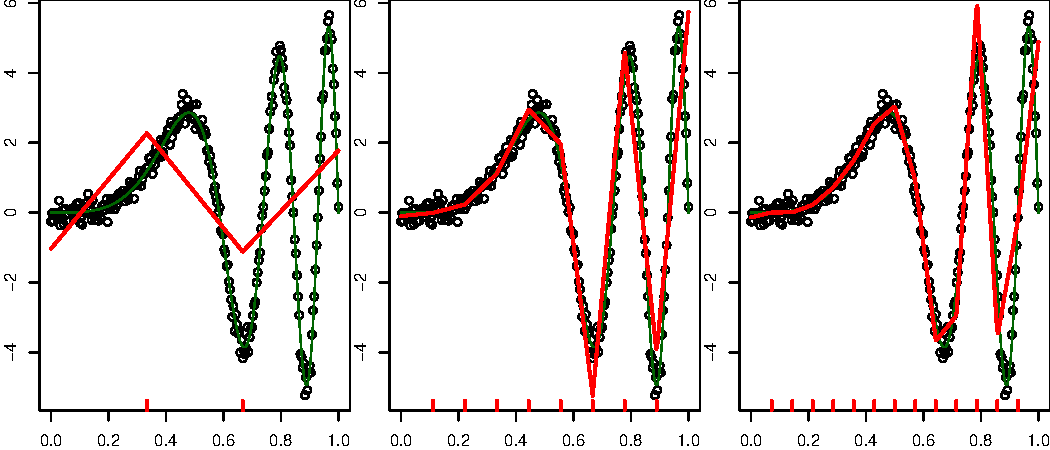
\includegraphics[width=0.9\textwidth]{figure/020-regression-1unnamed-chunk-20-1} 

\end{knitrout}
}
\onslide*<2>{
\begin{knitrout}
\definecolor{shadecolor}{rgb}{0.969, 0.969, 0.969}\color{fgcolor}
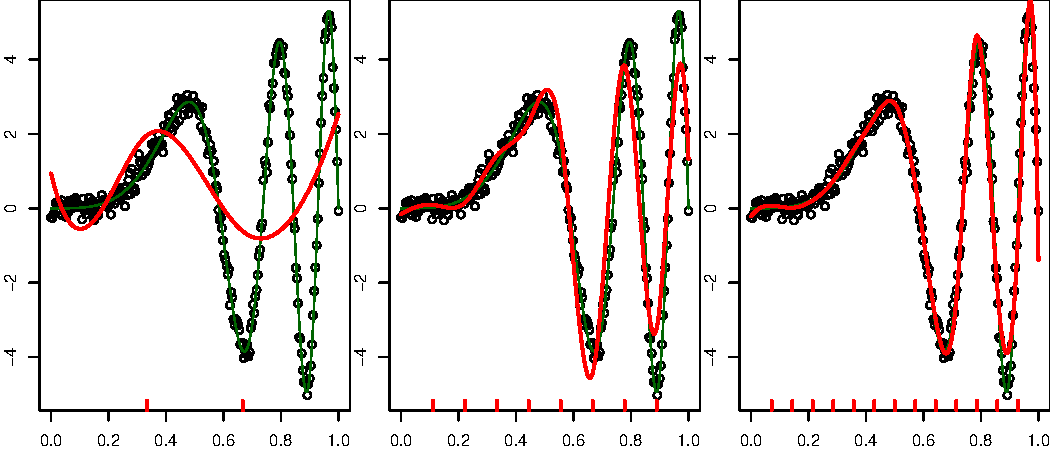
\includegraphics[width=0.9\textwidth]{figure/020-regression-1unnamed-chunk-21-1} 

\end{knitrout}
}


\end{center}
\end{frame}


\begin{frame}{Levigatezza della spline: nodi fissati}
Una strategia differente prevede di fissare i nodi e quindi
\begin{itemize}
\item[] imporre qualche restrizione sui coefficienti tale che cambiando la restrizione si cambi il grado di levigatezza.
\end{itemize}
o
\begin{itemize}
\item[] invece di stimare i coefficienti col metodo dei minimi quadrati, aggiungere una penalizzazione che favorisca funzioni pi\`u lisce.
\end{itemize}
Operando cos\`i, il grado di levigatezza dipende da un numero, che varia nel continuo.

%\spazio

%The second alternative leads to the idea of penalized sum of squares. (Note that it is equivalent to the first for some choices of constraint/penalization.)

\end{frame}




\section[Penalizzazione]{Verosimiglianza (somma dei quadrati) penalizzata}

\begin{frame}{Penalizzazione per la ruvidit\`a}
Dati i nodi e quindi una base, i parametri sono determinati minimizzando
\[ \sum_{i=1}^n (y_i-f(x_i,\vbeta,\vb))^2 + \lambda S(f(x,\vbeta,\vb)) \]
dove 
\begin{itemize}
\item $S(f(x,\vbeta,\vb))$ \`e una misura di quanto ``ruvida'' \`e $f()$, 
\item $\lambda>0$ \`e (almeno per ora) una costante fissata.
\end{itemize}
\end{frame}


\begin{frame}{Penalizzazione: tipo ridge}
Una penalizzazione semplice \`e data da
\[ S(f(x)) = \sum_{i=1}^K b_i^2 = \vb^T\vb \]
Si pu\`o mostrare che usare una penalizzazione di questo tipo equivale a porre un vincolo del tipo
\[ \sum_{i=1}^Kb_i^2<C \]
per qualche $C$.
\end{frame}



\begin{frame}[fragile]{TPB in notazione matriciale}
Consideriamo la base delle potenze troncate
\[ f(x) = \beta_1+\beta_2 x + \ldots + \beta_{p+1}x^p + \sum_{k=1}^K b_k (x-\nu_k)_+^p \]
e poniamo 
\begin{scriptsize}
\[
{\bm\theta}=\begin{bmatrix} \beta_1 \\ \vdots \\ \beta_{p+1} \\ b_1 \\ \vdots \\ b_K \end{bmatrix},\;\;\;\;
X=\begin{bmatrix}
1 & x_1 & x_1^2 & x_1^3 & (x_1-\nu_1)_+^3 & \ldots & (x_1-\nu_K)_+^3 \\
\vdots & \vdots & \vdots & \vdots & \vdots & \ddots & \vdots & \\
1 & x_i & x_i^2 & x_i^3 & (x_i-\nu_1)_+^3 & \ldots & (x_i-\nu_K)_+^3 \\
\vdots & \vdots & \vdots & \vdots & \vdots & \ddots & \vdots & \\
1 & x_n & x_n^2 & x_n^3 & (x_n-\nu_1)_+^3 & \ldots & (x_n-\nu_K)_+^3 
\end{bmatrix}
\]
\end{scriptsize}
Quindi $f({\bf x})=X{\bm\theta}$ e il modello \`e
\[ {\bf y} = X{\bm\theta} + {\bm\varepsilon}  \]
\end{frame}

\begin{frame}[fragile]{Penalizzazione e TPB}
Considerimao la penalizzazione ridge
\[ S(f(x,{\bm\theta})) = {\bm\theta}^TD{\bm\theta} \]
dove $D=\text{diag}(0_{p+1},1_K)$,

\spazio

Il minimo di
\[ \sum_{i=1}^n(y_i-f(x_i,{\bm\theta}))^2 - \lambda{\bm\theta}^TD{\bm\theta}  \]
si ha per
\[ {\bm\hat\theta} = (X^TX+\lambda D)^{-1}X^Ty \]
Quindi la spline, scritta in forma di lisciatore lineare, \`e
\[ \hat{y} = X(X^TX+\lambda D)^{-1}X^Ty \]
\end{frame}

\begin{frame}{Quanti sono i parametri?}
``Nominalmente'' il modello ha $K+p+1$ parametri (e la varianza)

\spazio

Per\`o, questi non possono variare liberamente per via della penalizzazione.

\spazio

Il numero effettivo di parametri \`e valutato come la traccia della matrice di lisciamento
\[ \mbox{trace}(X(X^TX+\lambda D)^{-1}X^T) \]

\spazio

(Analogamente, si ricordi che nel ML, il numero di parametri \`e la traccia della matrice di proiezione.)

\end{frame}

\begin{frame}{Penalizzazione: derivata seconda}
Un'alternativa \`e impiegare una derivata della funzione spline
\[ S(f(x)) = \int (f^{(q)}(t))^2dt \]
dove $q\leq\mbox{grado della spline}$. (In genere $q=2$ per una spline cubica.)

Si noti che, se la base \`e ${\bf B}() = (B_1(),\ldots,B_K())$, sicch\`e
\[ \hat{f}(x) = {\bm{b}}^T{\bf B}(x) \]
allora 
\[ S(f(x)) = \int (f^{(q)}(t))^2dt = {\bm{b}}^TD{\bm{b}} \]
dove
\[ D = \int_a^b  {\bf B}^{(q)}(x)[{\bf B}^{(q)}(x)]^Tdx \]
(In certi casi  si usano approssimazioni.)
\end{frame}


\begin{frame}{Funzioni e le loro derivate seconde}
Si riportano tre funzioni e i quadrati delle derivate seconde.
\begin{center}
\begin{knitrout}
\definecolor{shadecolor}{rgb}{0.969, 0.969, 0.969}\color{fgcolor}
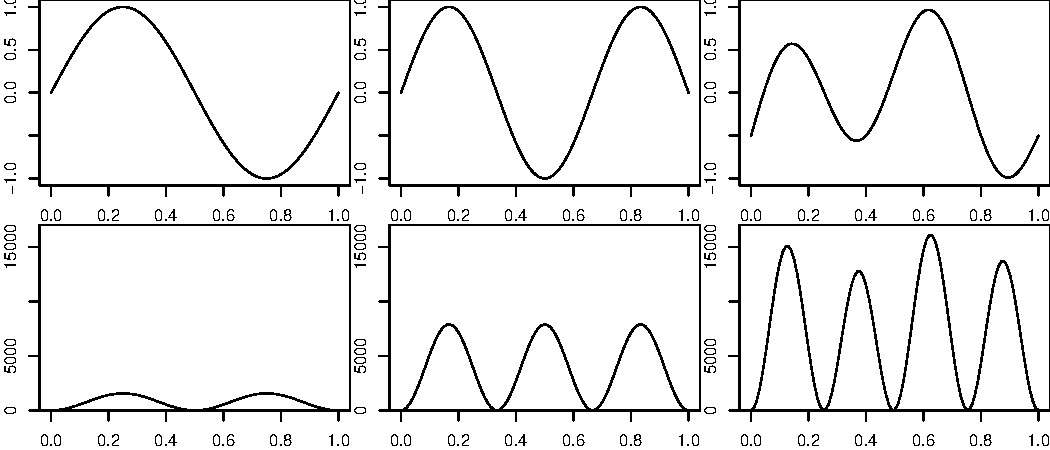
\includegraphics[width=0.9\textwidth]{figure/020-regression-1unnamed-chunk-22-1} 

\end{knitrout}
\end{center}
\end{frame}




\begin{frame}[fragile]{Spline penalizzate}
\begin{columns}
\column{0.7\textwidth}
\begin{knitrout}
\definecolor{shadecolor}{rgb}{0.969, 0.969, 0.969}\color{fgcolor}\begin{kframe}


{\ttfamily\noindent\bfseries\color{errorcolor}{Error in plot(lidar\$range, lidar\$logratio, pch = 20, xlab = "{}x"{}, ylab = "{}y"{}, : oggetto "{}lidar"{} non trovato}}

{\ttfamily\noindent\bfseries\color{errorcolor}{Error in lines(lidar\$range, y.teo(lidar\$logratio, lidar\$range, l = 0, : oggetto "{}lidar"{} non trovato}}

{\ttfamily\noindent\bfseries\color{errorcolor}{Error in lines(lidar\$range, y.teo(lidar\$logratio, lidar\$range, l = 0.001, : oggetto "{}lidar"{} non trovato}}

{\ttfamily\noindent\bfseries\color{errorcolor}{Error in lines(lidar\$range, y.teo(lidar\$logratio, lidar\$range, l = 1e-05, : oggetto "{}lidar"{} non trovato}}

{\ttfamily\noindent\bfseries\color{errorcolor}{Error in seq(min(lidar\$range), max(lidar\$range), length = 40 + 2): oggetto "{}lidar"{} non trovato}}

{\ttfamily\noindent\bfseries\color{errorcolor}{Error in strwidth(legend, units = "{}user"{}, cex = cex, font = text.font): plot.new has not been called yet}}\end{kframe}
\end{knitrout}
\column{0.3\textwidth}
Nel grafico si riportano 3 spline stimate usando 40 nodi con diversi pesi per la penalizzazione (tipo ridge).
\end{columns}
\end{frame}



\begin{frame}[fragile]{Spline penalizzate e non}
\begin{knitrout}
\definecolor{shadecolor}{rgb}{0.969, 0.969, 0.969}\color{fgcolor}







































\animategraphics[width=0.95\textwidth,height=0.8\textheight,controls,loop]{1}{figure/020-regression-1knotseffectANpenunpen-}{1}{40}

\end{knitrout}
\end{frame}



\begin{frame}[fragile]{Quindi quanti nodi?}
Il trucco della penalizzazione fa s\`i che possiamo fissare i nodi all'inizio, come per\`o?
\begin{itemize}
\item L'idea \`e che, siccome si usa la penalizzazione, la scelta dei nodi \`e poco importante purch\'e
\begin{itemize}
\item non siano troppo pochi (in generale: da 20 a 40 minimo),
\item ci siano osservazioni tra i nodi (almeno 4-5 osservazioni tra uno e l'altro)
\end{itemize}
\item Si possono fissare tanti nodi quante le osservazioni, pu\`o essere per\`o computazionalmente oneroso e, in genere, non \`e necessario.
\item Strategie tipiche per la scelta della posizione dei nodi sono
\begin{itemize}
\item quantili empirici di $x$ 
\item nodi equispaziati.
\end{itemize}
\end{itemize}

\begin{center}
{\bf Da qui in poi, i nodi $\nu_1,\ldots, \nu_K$ sono fissati in qualche modo.}
\end{center}

(Si noti che possiamo verificare se i nodi sono in numero sufficiente stimando il modello con un numero maggiore e verificando se le cose cambiano.)
\end{frame}









%%%%%%%%%%%%%%%%%%%%%%%%%%%%%%%%%%%%%%%%%%%%%%%%%%%%%%%%%%%%%%%
%%%%%%%%%%%%%%%%%%%%%%%%%%%%%%%%%%%%%%%%%%%%%%%%%%%%%%%%%%%%%%%

\subsection{Scelta di $\lambda$}

\begin{frame}{Scelta di $\lambda$}
Il ruolo di $\lambda$ \`e analogo alla scelta del numero di vicini o della banda.

\spazio

Lo stesso criterio: validazione incrociata, pu\`o essere impiegato per la scelta.

\spazio

Si noti che la spline \`e un lisciatore lineare, quindi i risultati visti in generale per i lisciatori lineari si possono impiegare anche ora.

\spazio

Inotlre, anche la formula per il GCV \`e valida.
\end{frame}


\begin{frame}{Errore quadratico complessivo}
\onslide*<1>{
Let 
\begin{eqnarray*} 
\mbox{R}(\hat{f}) &=& E\left(\sum_{i=1}^n (\hat{f}(x_i)-f(x_i))^2 \right)    \\
&=& \sum_{i=1}^n [(E(\hat{f}(x_i))-f(x_i))^2 + V(\hat{f}(x_i))] \\
&=& (E(L{\bm y})-{\bm f})^T(E(L{\bm y})-{\bm f}) + \sum_{i=1}^n V(L{\bm y})_{ii} \\
&=& {\bm f}^T(L-I)^T(L-I){\bm f}  + \mbox{trace}[V(L{\bm y})] \\
&=& {\bm f}^T(L-I)^T(L-I){\bm f}  + \mbox{trace}[LV({\bm y})L^T] \\
&=& {\bm f}^T(L-I)^T(L-I){\bm f}  + \sigma^2_{\varepsilon}\mbox{trace}[LL^T]
\end{eqnarray*}
In questa scomposizione, la prima parte rappresenta il quadrato della distorsione, la seconda \`e la varianza.
}

\onslide*<2>{
\begin{center}
Esempio di scomposizione di R in distorsione e varianza

\begin{tabular}{cc}
\begin{knitrout}
\definecolor{shadecolor}{rgb}{0.969, 0.969, 0.969}\color{fgcolor}
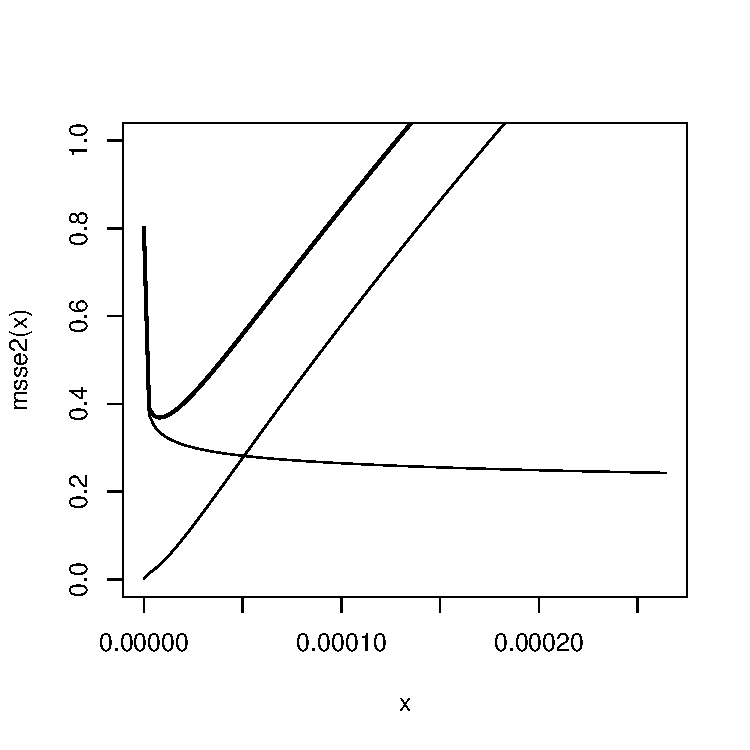
\includegraphics[width=0.45\textwidth]{figure/020-regression-1aa-1} 

\end{knitrout}

&

\begin{knitrout}
\definecolor{shadecolor}{rgb}{0.969, 0.969, 0.969}\color{fgcolor}
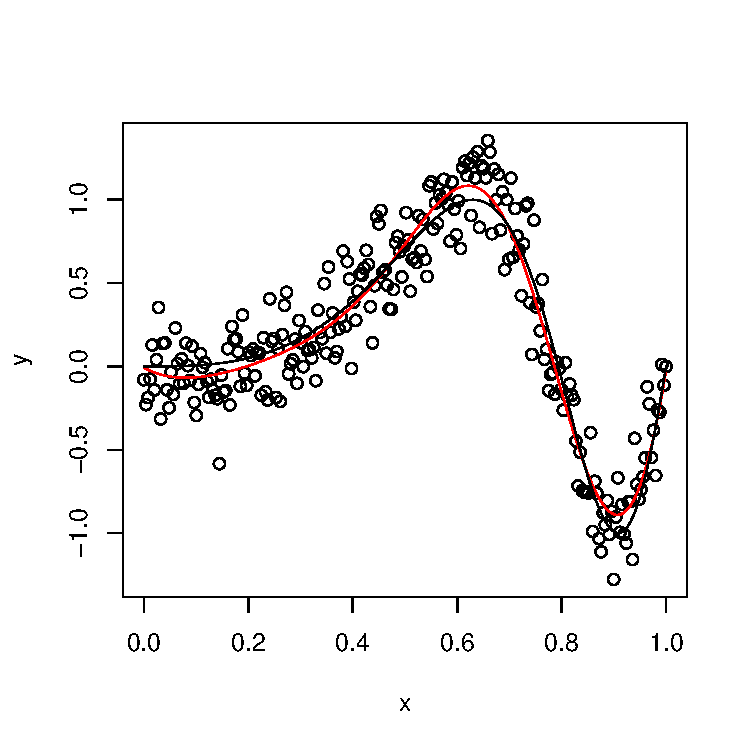
\includegraphics[width=0.45\textwidth]{figure/020-regression-1unnamed-chunk-24-1} 

\end{knitrout}
\end{tabular}
\end{center}

}

\end{frame}

\begin{frame}{Gradi di libert\`a e penalizzazione}
Il coefficiente $\lambda$ determina la levigatezza della funzione stimata, \`e rilevante studiare come variano i gradi di libert\`a di $\hat{f}$ ( $\mbox{df}=\mbox{tr}(L)$) in funzione di $\lambda$.

\begin{knitrout}
\definecolor{shadecolor}{rgb}{0.969, 0.969, 0.969}\color{fgcolor}

{\centering 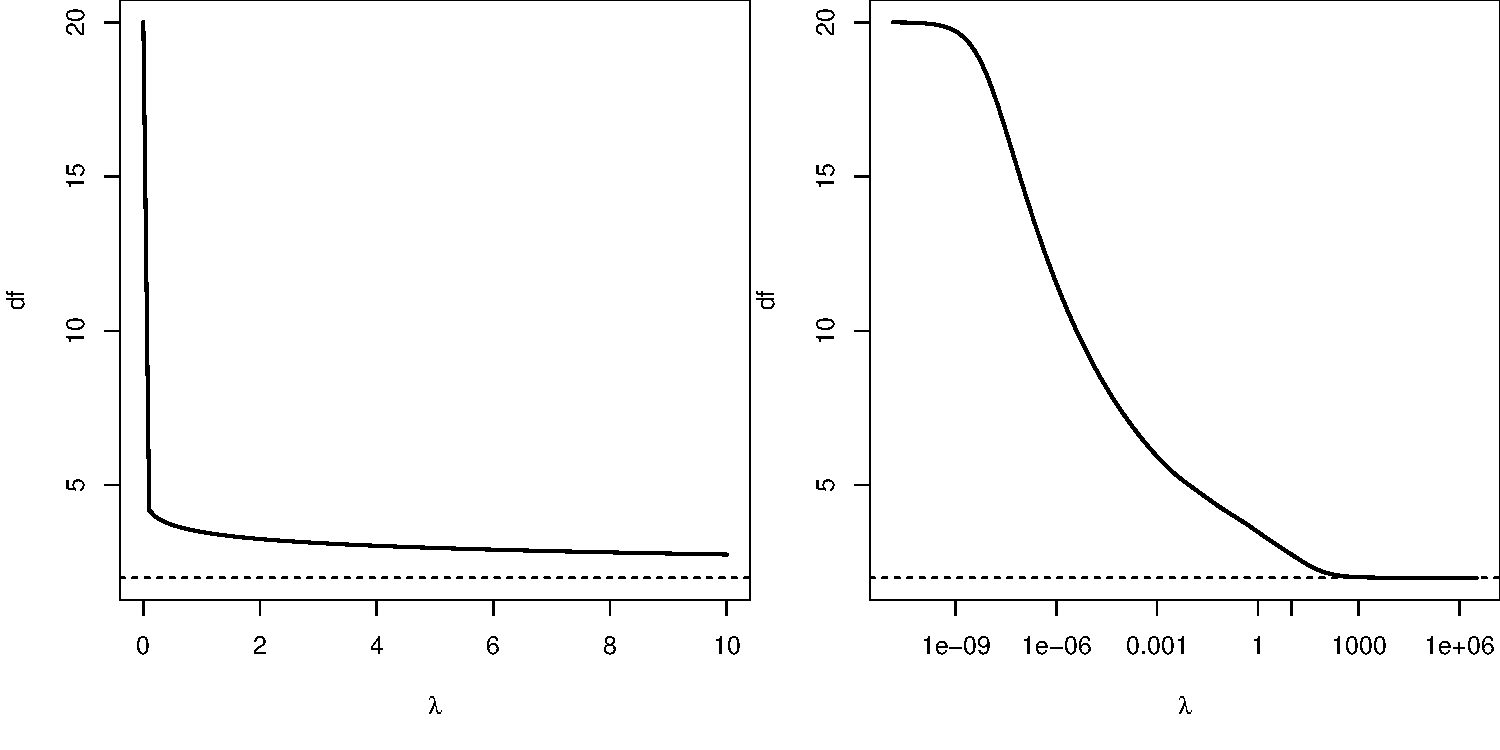
\includegraphics[width=0.9\textwidth]{figure/020-regression-1unnamed-chunk-25-1} 

}



\end{knitrout}


\end{frame}



\begin{frame}[fragile]{Spline in R: {\tt gam} ({\tt mgcv})}
ci sono numerosi pacchetti per la stima di spline in R, uno dei pi\`u potenti e versatili \`e il pacchetto {\tt mgcv} di Wood.

\spazio

Le funzioni del pacchetto presentano molte opsioni, nella forma pi\`u semplice, comunque:

\begin{knitrout}
\definecolor{shadecolor}{rgb}{0.969, 0.969, 0.969}\color{fgcolor}\begin{kframe}
\begin{alltt}
\hlstd{fit}\hlkwb{=}\hlkwd{gam}\hlstd{(y}\hlopt{~}\hlkwd{s}\hlstd{(x))}
\hlstd{fit.s}\hlkwb{=}\hlkwd{summary}\hlstd{(fit)}
\hlkwd{plot}\hlstd{(fit)}
\end{alltt}
\end{kframe}
\end{knitrout}

si effettua una stima scegliendo via GCV il parametro di lisciamento $\lambda$ (la scelta dei nodi \`e fatta in maniera predefinita di cui non ci preoccupiamo, volendo si possono cambiare).
\end{frame}

\begin{frame}[fragile]{Stimare una spline con {\tt gam}}
Tra gli argomenti della funzione {\tt s()}
\begin{itemize}
\item[k] dimensione della base
\item[fx] se usare una penalizzazione
\end{itemize}

\begin{knitrout}
\definecolor{shadecolor}{rgb}{0.969, 0.969, 0.969}\color{fgcolor}\begin{kframe}
\begin{alltt}
\hlstd{fit2}\hlkwb{=}\hlkwd{gam}\hlstd{(y}\hlopt{~}\hlkwd{s}\hlstd{(x,}\hlkwc{k}\hlstd{=}\hlnum{3}\hlstd{))}
\hlstd{fit4}\hlkwb{=}\hlkwd{gam}\hlstd{(y}\hlopt{~}\hlkwd{s}\hlstd{(x,}\hlkwc{k}\hlstd{=}\hlnum{10}\hlstd{))}
\hlkwd{plot}\hlstd{(fit2)}
\hlkwd{plot}\hlstd{(fit8)}
\end{alltt}
\end{kframe}
\end{knitrout}

\end{frame}

\begin{frame}[fragile]{LIDAR: GAM}

\begin{center}
\begin{scriptsize}
\begin{knitrout}
\definecolor{shadecolor}{rgb}{0.969, 0.969, 0.969}\color{fgcolor}\begin{kframe}
\begin{alltt}
\hlkwd{plot}\hlstd{(lidar}\hlopt{$}\hlstd{range,lidar}\hlopt{$}\hlstd{logratio,}\hlkwc{pch}\hlstd{=}\hlnum{20}\hlstd{,}\hlkwc{xlab}\hlstd{=}\hlstr{"x"}\hlstd{,}\hlkwc{ylab}\hlstd{=}\hlstr{"y"}\hlstd{,}\hlkwc{ylim}\hlstd{=}\hlkwd{c}\hlstd{(}\hlopt{-}\hlnum{1}\hlstd{,}\hlnum{0.2}\hlstd{))}
\end{alltt}


{\ttfamily\noindent\bfseries\color{errorcolor}{Error in plot(lidar\$range, lidar\$logratio, pch = 20, xlab = "{}x"{}, ylab = "{}y"{}, : oggetto "{}lidar"{} non trovato}}\end{kframe}
\end{knitrout}
\end{scriptsize}
\end{center}

\end{frame}


\begin{frame}[fragile]{LIDAR: GAM}

\begin{center}
\begin{scriptsize}
\begin{knitrout}
\definecolor{shadecolor}{rgb}{0.969, 0.969, 0.969}\color{fgcolor}\begin{kframe}
\begin{alltt}
\hlstd{fit}\hlkwb{=}\hlkwd{gam}\hlstd{(logratio}\hlopt{~}\hlkwd{s}\hlstd{(range),}\hlkwc{data}\hlstd{=lidar)}
\end{alltt}


{\ttfamily\noindent\bfseries\color{errorcolor}{Error in is.data.frame(data): oggetto "{}lidar"{} non trovato}}\begin{alltt}
\hlkwd{plot}\hlstd{(fit)}
\end{alltt}
\end{kframe}
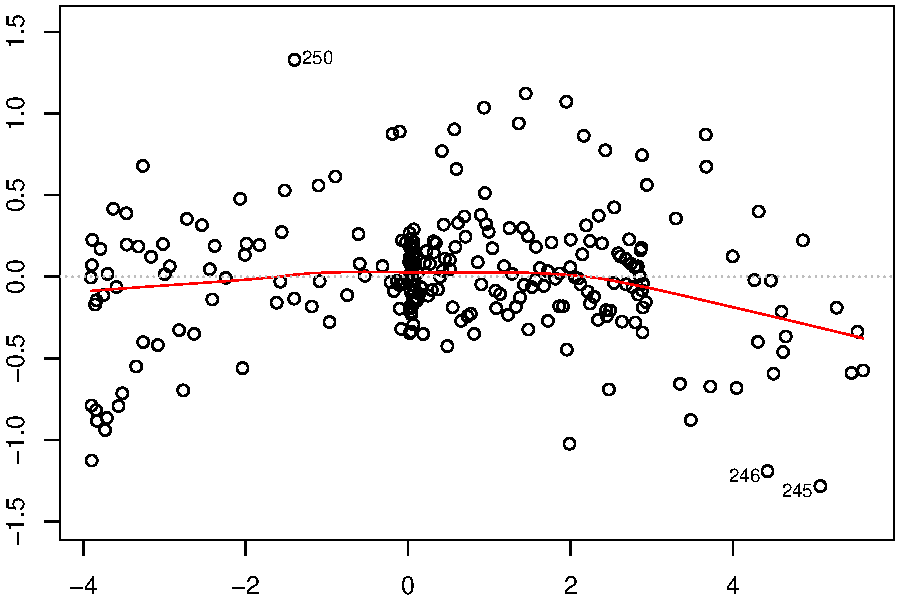
\includegraphics[width=0.7\textwidth]{figure/020-regression-1unnamed-chunk-29-1} 

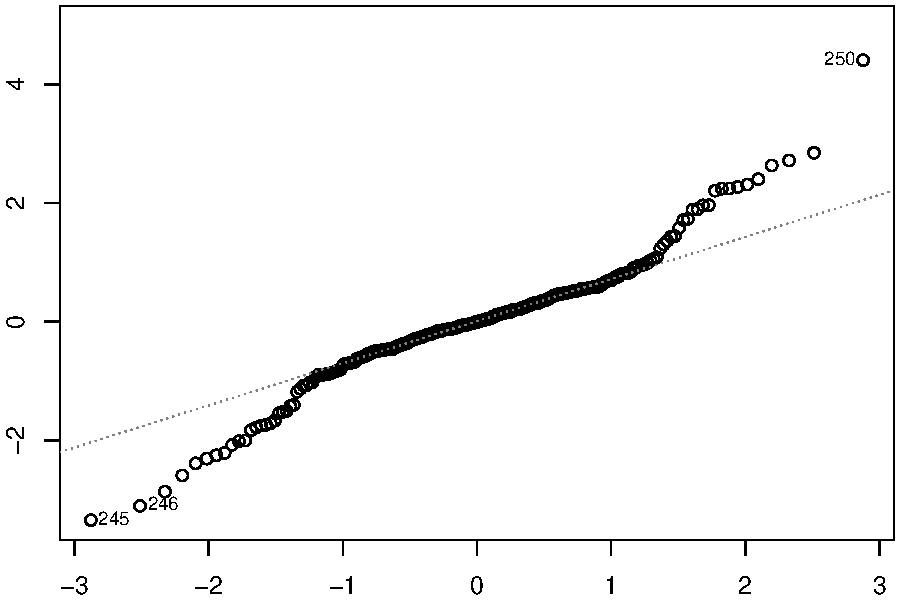
\includegraphics[width=0.7\textwidth]{figure/020-regression-1unnamed-chunk-29-2} 

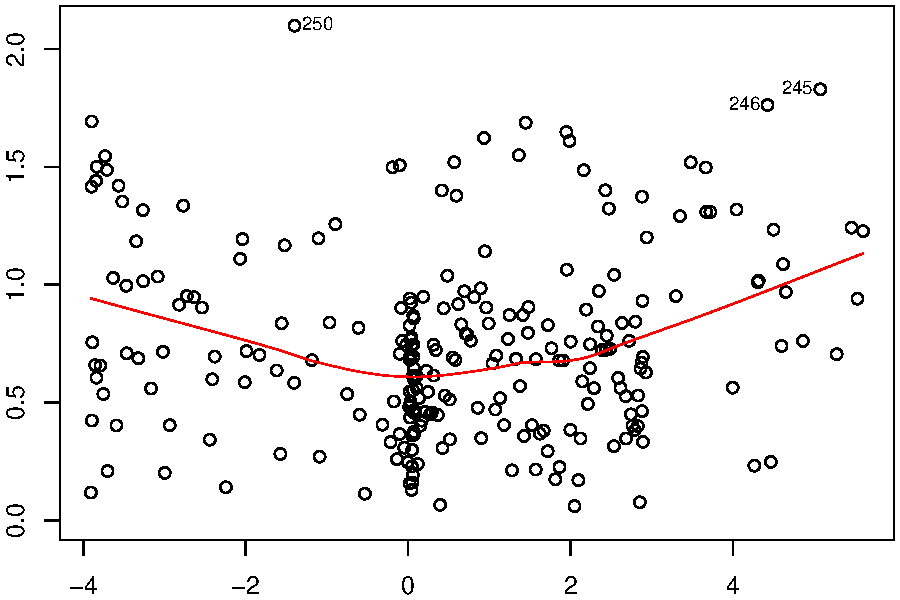
\includegraphics[width=0.7\textwidth]{figure/020-regression-1unnamed-chunk-29-3} 

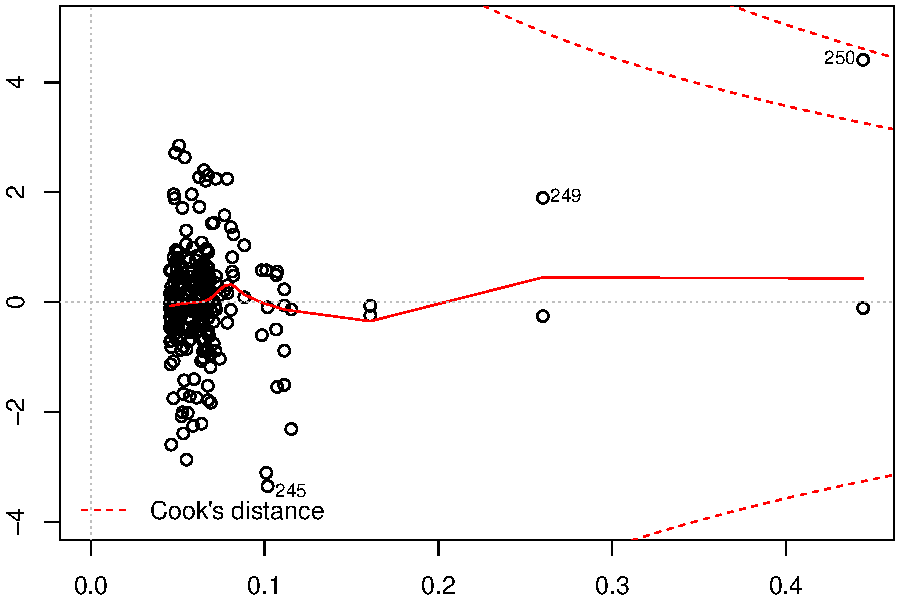
\includegraphics[width=0.7\textwidth]{figure/020-regression-1unnamed-chunk-29-4} 

\end{knitrout}
\end{scriptsize}
\end{center}

\end{frame}

\begin{frame}[fragile]{LIDAR: GAM}

\begin{center}
\begin{scriptsize}
\begin{knitrout}
\definecolor{shadecolor}{rgb}{0.969, 0.969, 0.969}\color{fgcolor}\begin{kframe}
\begin{alltt}
\hlkwd{plot}\hlstd{(lidar}\hlopt{$}\hlstd{range,lidar}\hlopt{$}\hlstd{logratio,}\hlkwc{pch}\hlstd{=}\hlnum{20}\hlstd{,}\hlkwc{xlab}\hlstd{=}\hlstr{"x"}\hlstd{,}\hlkwc{ylab}\hlstd{=}\hlstr{"y"}\hlstd{,}\hlkwc{ylim}\hlstd{=}\hlkwd{c}\hlstd{(}\hlopt{-}\hlnum{1}\hlstd{,}\hlnum{0.2}\hlstd{))}
\end{alltt}


{\ttfamily\noindent\bfseries\color{errorcolor}{Error in plot(lidar\$range, lidar\$logratio, pch = 20, xlab = "{}x"{}, ylab = "{}y"{}, : oggetto "{}lidar"{} non trovato}}\begin{alltt}
\hlkwd{curve}\hlstd{(}\hlkwd{predict}\hlstd{(fit,}\hlkwc{newdata}\hlstd{=}\hlkwd{data.frame}\hlstd{(}\hlkwc{range}\hlstd{=x)),}\hlkwc{add}\hlstd{=}\hlnum{TRUE}\hlstd{)}
\end{alltt}


{\ttfamily\noindent\color{warningcolor}{Warning: 'newdata' had 101 rows but variables found have 250 rows}}

{\ttfamily\noindent\bfseries\color{errorcolor}{Error: variable 'X' was fitted with type "{}nmatrix.17"{} but type "{}nmatrix.20"{} was supplied}}\end{kframe}
\end{knitrout}
\end{scriptsize}
\end{center}

\end{frame}

\begin{frame}[fragile]{LIDAR: GAM}

\begin{center}
\begin{scriptsize}
\begin{knitrout}
\definecolor{shadecolor}{rgb}{0.969, 0.969, 0.969}\color{fgcolor}\begin{kframe}
\begin{alltt}
\hlkwd{plot}\hlstd{(lidar}\hlopt{$}\hlstd{range,lidar}\hlopt{$}\hlstd{logratio,}\hlkwc{pch}\hlstd{=}\hlnum{20}\hlstd{,}\hlkwc{xlab}\hlstd{=}\hlstr{"x"}\hlstd{,}\hlkwc{ylab}\hlstd{=}\hlstr{"y"}\hlstd{,}\hlkwc{ylim}\hlstd{=}\hlkwd{c}\hlstd{(}\hlopt{-}\hlnum{1}\hlstd{,}\hlnum{0.2}\hlstd{))}
\end{alltt}


{\ttfamily\noindent\bfseries\color{errorcolor}{Error in plot(lidar\$range, lidar\$logratio, pch = 20, xlab = "{}x"{}, ylab = "{}y"{}, : oggetto "{}lidar"{} non trovato}}\begin{alltt}
\hlstd{xx}\hlkwb{=}\hlkwd{seq}\hlstd{(}\hlkwd{min}\hlstd{(lidar}\hlopt{$}\hlstd{range),}\hlkwd{max}\hlstd{(lidar}\hlopt{$}\hlstd{range),}\hlkwc{length}\hlstd{=}\hlnum{100}\hlstd{)}
\end{alltt}


{\ttfamily\noindent\bfseries\color{errorcolor}{Error in seq(min(lidar\$range), max(lidar\$range), length = 100): oggetto "{}lidar"{} non trovato}}\begin{alltt}
\hlstd{pr}\hlkwb{=}\hlkwd{predict}\hlstd{(fit,}\hlkwc{newdata}\hlstd{=}\hlkwd{data.frame}\hlstd{(}\hlkwc{range}\hlstd{=xx),}
              \hlkwc{se.fit}\hlstd{=}\hlnum{TRUE}\hlstd{)}
\end{alltt}


{\ttfamily\noindent\bfseries\color{errorcolor}{Error in data.frame(range = xx): oggetto "{}xx"{} non trovato}}\begin{alltt}
\hlkwd{matlines}\hlstd{(xx,}\hlkwd{cbind}\hlstd{(pr}\hlopt{$}\hlstd{fit}\hlopt{-}\hlnum{2}\hlopt{*}\hlstd{pr}\hlopt{$}\hlstd{se.fit,pr}\hlopt{$}\hlstd{fit,pr}\hlopt{$}\hlstd{fit}\hlopt{+}\hlnum{2}\hlopt{*}\hlstd{pr}\hlopt{$}\hlstd{se.fit),}
        \hlkwc{type}\hlstd{=}\hlstr{"l"}\hlstd{,}\hlkwc{lty}\hlstd{=}\hlkwd{c}\hlstd{(}\hlnum{2}\hlstd{,}\hlnum{1}\hlstd{,}\hlnum{2}\hlstd{),}\hlkwc{col}\hlstd{=}\hlstr{"black"}\hlstd{)}
\end{alltt}


{\ttfamily\noindent\bfseries\color{errorcolor}{Error in as.matrix(x): oggetto "{}xx"{} non trovato}}\end{kframe}
\end{knitrout}
\end{scriptsize}
\end{center}

\end{frame}


\begin{frame}[fragile]{LIDAR: GAM}

\begin{center}
\begin{tiny}
\begin{knitrout}
\definecolor{shadecolor}{rgb}{0.969, 0.969, 0.969}\color{fgcolor}\begin{kframe}
\begin{alltt}
\hlkwd{summary}\hlstd{(fit)}
\end{alltt}
\begin{verbatim}

Call:
lm(formula = y ~ X - 1)

Residuals:
     Min       1Q   Median       3Q      Max 
-1.28339 -0.18430 -0.00155  0.18844  1.32864 

Coefficients:
      Estimate Std. Error t value Pr(>|t|)    
X1  -2.170e-01  2.697e-01  -0.805  0.42189    
X2   1.072e+01  2.141e+01   0.501  0.61690    
X3  -1.269e+02  4.453e+02  -0.285  0.77587    
X4   4.640e+02  2.605e+03   0.178  0.85879    
X5  -1.668e+02  3.447e+03  -0.048  0.96145    
X6  -3.309e+02  1.623e+03  -0.204  0.83867    
X7   9.002e+01  1.343e+03   0.067  0.94660    
X8  -3.024e+02  1.272e+03  -0.238  0.81228    
X9   3.789e+02  1.252e+03   0.302  0.76254    
X10 -1.738e+03  1.247e+03  -1.394  0.16468    
X11  2.158e+03  1.246e+03   1.732  0.08458 .  
X12  1.732e+03  1.247e+03   1.389  0.16616    
X13  3.758e+03  1.252e+03   3.001  0.00299 ** 
X14 -2.627e+04  1.272e+03 -20.654  < 2e-16 ***
X15  3.908e+04  1.343e+03  29.109  < 2e-16 ***
X16 -1.315e+04  1.623e+03  -8.098 3.11e-14 ***
X17 -7.578e+04  3.447e+03 -21.983  < 2e-16 ***
---
Signif. codes:  
0 '***' 0.001 '**' 0.01 '*' 0.05 '.' 0.1 ' ' 1

Residual standard error: 0.4045 on 233 degrees of freedom
Multiple R-squared:  0.9715,	Adjusted R-squared:  0.9694 
F-statistic: 467.1 on 17 and 233 DF,  p-value: < 2.2e-16
\end{verbatim}
\end{kframe}
\end{knitrout}
\end{tiny}
\end{center}

\end{frame}

\begin{frame}[fragile]{LIDAR: GAM}

\begin{center}
\begin{scriptsize}
\begin{knitrout}
\definecolor{shadecolor}{rgb}{0.969, 0.969, 0.969}\color{fgcolor}\begin{kframe}
\begin{alltt}
\hlkwd{plot}\hlstd{(lidar}\hlopt{$}\hlstd{range,lidar}\hlopt{$}\hlstd{logratio,}\hlkwc{pch}\hlstd{=}\hlnum{20}\hlstd{,}\hlkwc{xlab}\hlstd{=}\hlstr{"x"}\hlstd{,}\hlkwc{ylab}\hlstd{=}\hlstr{"y"}\hlstd{,}\hlkwc{ylim}\hlstd{=}\hlkwd{c}\hlstd{(}\hlopt{-}\hlnum{1}\hlstd{,}\hlnum{0.2}\hlstd{))}
\end{alltt}


{\ttfamily\noindent\bfseries\color{errorcolor}{Error in plot(lidar\$range, lidar\$logratio, pch = 20, xlab = "{}x"{}, ylab = "{}y"{}, : oggetto "{}lidar"{} non trovato}}\begin{alltt}
\hlkwd{curve}\hlstd{(}\hlkwd{predict}\hlstd{(fit,}\hlkwc{newdata}\hlstd{=}\hlkwd{data.frame}\hlstd{(}\hlkwc{range}\hlstd{=x)),}\hlkwc{add}\hlstd{=}\hlnum{TRUE}\hlstd{)}
\end{alltt}


{\ttfamily\noindent\color{warningcolor}{Warning: 'newdata' had 101 rows but variables found have 250 rows}}

{\ttfamily\noindent\bfseries\color{errorcolor}{Error: variable 'X' was fitted with type "{}nmatrix.17"{} but type "{}nmatrix.20"{} was supplied}}\begin{alltt}
\hlstd{fit1}\hlkwb{=}\hlkwd{gam}\hlstd{(logratio}\hlopt{~}\hlkwd{s}\hlstd{(range,}\hlkwc{fx}\hlstd{=}\hlnum{TRUE}\hlstd{,}\hlkwc{k}\hlstd{=}\hlnum{3}\hlstd{),}\hlkwc{data}\hlstd{=lidar)}
\end{alltt}


{\ttfamily\noindent\bfseries\color{errorcolor}{Error in is.data.frame(data): oggetto "{}lidar"{} non trovato}}\begin{alltt}
\hlkwd{curve}\hlstd{(}\hlkwd{predict}\hlstd{(fit1,}\hlkwc{newdata}\hlstd{=}\hlkwd{data.frame}\hlstd{(}\hlkwc{range}\hlstd{=x)),}\hlkwc{add}\hlstd{=}\hlnum{TRUE}\hlstd{,}\hlkwc{col}\hlstd{=}\hlstr{"red"}\hlstd{)}
\end{alltt}


{\ttfamily\noindent\bfseries\color{errorcolor}{Error in predict(fit1, newdata = data.frame(range = x)): oggetto "{}fit1"{} non trovato}}\end{kframe}
\end{knitrout}
\end{scriptsize}
\end{center}

\end{frame}



\begin{frame}[fragile]{Qualche esperimento con {\tt gam}}
``Verifichiamo'' che il numero di nodi \`e indifferente purch\'e abbastanza grande.
The number of knots does not matter provided it is high enough.

\begin{knitrout}
\definecolor{shadecolor}{rgb}{0.969, 0.969, 0.969}\color{fgcolor}\begin{kframe}
\begin{alltt}
\hlstd{sim}\hlkwb{=}\hlkwd{data.frame}\hlstd{(}\hlkwc{x}\hlstd{=}\hlkwd{seq}\hlstd{(}\hlnum{0}\hlstd{,}\hlnum{1}\hlstd{,}\hlkwc{length}\hlstd{=}\hlnum{200}\hlstd{))} \hlcom{#sort(runif(150,0,1)))}
\hlstd{sim}\hlopt{$}\hlstd{m}\hlkwb{=}\hlkwd{sin}\hlstd{(}\hlnum{2}\hlopt{*}\hlstd{pi}\hlopt{*}\hlstd{sim}\hlopt{$}\hlstd{x}\hlopt{^}\hlnum{3}\hlstd{)}
\hlstd{sim}\hlopt{$}\hlstd{y}\hlkwb{=}\hlstd{sim}\hlopt{$}\hlstd{m}\hlopt{+}\hlkwd{rnorm}\hlstd{(}\hlkwd{nrow}\hlstd{(sim),}\hlnum{0}\hlstd{,}\hlnum{0.4}\hlstd{)}
\hlkwd{plot}\hlstd{(sim}\hlopt{$}\hlstd{x,sim}\hlopt{$}\hlstd{y)}
\hlstd{fit0}\hlkwb{=}\hlkwd{gam}\hlstd{(y}\hlopt{~}\hlkwd{s}\hlstd{(x),}\hlkwc{data}\hlstd{=sim)}
\hlstd{fit1}\hlkwb{=}\hlkwd{gam}\hlstd{(y}\hlopt{~}\hlkwd{s}\hlstd{(x,}\hlkwc{k}\hlstd{=}\hlnum{5}\hlstd{),}\hlkwc{data}\hlstd{=sim)}
\hlstd{fit2}\hlkwb{=}\hlkwd{gam}\hlstd{(y}\hlopt{~}\hlkwd{s}\hlstd{(x,}\hlkwc{k}\hlstd{=}\hlnum{12}\hlstd{),}\hlkwc{data}\hlstd{=sim)}
\hlstd{fit3}\hlkwb{=}\hlkwd{gam}\hlstd{(y}\hlopt{~}\hlkwd{s}\hlstd{(x,}\hlkwc{k}\hlstd{=}\hlnum{30}\hlstd{),}\hlkwc{data}\hlstd{=sim)}
\end{alltt}
\end{kframe}
\end{knitrout}

\end{frame}


\subsection{Perch\'e le spline}

\begin{frame}{Spline}

\begin{columns}

\column{0.5\textwidth}
Una spline di ordine $p$ con nodi $\nu_1,\ldots,\nu_K$ \`e un polinomio a tratti continuo con derivate continue fino all'ordine $p-1$.

\spazio

Il termine spline deriva dal nome di un attrezzo da disegno (una striscia di metallo flessibile usata per agevolare il disegno di curve).

\spazio

Una {\bf spline cubica} \`e una spline di ordine $p=3$ (continua con derivata seconda continua).

\column{0.05\textwidth}
\column{0.45\textwidth}



{\centering \includegraphics[width=0.75\textwidth]{figure/splinephys}


}

\begin{scriptsize}
A spline, or the more modern term flexible curve, consists of a long strip fixed in position at a number of points that relaxes to form and hold a smooth curve passing through those points for the purpose of transferring that curve to another material. (\href{https://en.wikipedia.org/wiki/Flat_spline}{Wikipedia})\par
\end{scriptsize}
\end{columns}
\end{frame}


\begin{frame}{Le spline naturali cubiche sono interpolanti ottimali}
Sia
\begin{itemize}
\item $(x_i,y_i)$, $i=1,\ldots,n$: dove $x_i<x_{i+1}$ 
\item $g(x)$ la spline cubica naturale che interpola i punti \\ (naturale significa che $g''(x_1)=g''(x_n)=0$)
\end{itemize}
allora $g()$ \`e l'interpolante pi\`u liscia nel senso che minimizza
\[ J(f) = \int_{x_1}^{x_n} f''(x)^2dx \]
tra le funzioni $f$ che interpolano i punti, sono assolutamente continue e hanno derivata prima continua.

\spazio

In altre parole, le spline cubiche naturali sono le funzioni pi\`u lisce per interpolare dei punti.
\end{frame}

\begin{frame}[t]{Dimostrazione}
Sia $f()$ interpolante $(x_i,y_i)$ e sia $h=f-g$
\begin{eqnarray*}
\int_{x_1}^{x_n}f''(x)^2dx 
\onslide*<1>{&=&  \int_{x_1}^{x_n}(g''(x)+h''(x))^2dx \\}
&=&  \int_{x_1}^{x_n}g''(x)^2dx + \int_{x_1}^{x_n}g''(x)h''(x)dx +\int_{x_1}^{x_n}h''(x)^2dx 
\end{eqnarray*}
\onslide*<2->{
Si ah anche, integrando per parti
\begin{align*}
\int_{x_1}^{x_n}g''(x)h''(x)dx 
\onslide*<2>{
&= g''(x_n)h'(x_n)-g''(x_1)h'(x_1) -  \int_{x_1}^{x_n}g'''(x)h'(x)dx  \\
%\intertext{si$g''(x_n)=g''(x_1)=0$}
& = -\int_{x_1}^{x_n}g'''(x)h'(x)dx  \\
&= -\sum_{i=1}^{n-1} g'''(x_i^+)\int_{x_1}^{x_n}h'(x)dx \\
&= -\sum_{i=1}^{n-1} g'''(x_i^+)(h(x_{i+1})-h(x_i))
} =0
\end{align*}
}
\onslide*<3>{
Quindi
\begin{eqnarray*}
\int_{x_1}^{x_n}f''(x)^2dx 
=  \int_{x_1}^{x_n}g''(x)^2dx +\int_{x_1}^{x_n}h''(x)^2dx \geq \int_{x_1}^{x_n}g''(x)^2dx
\end{eqnarray*}
dove si ha l'eguaglianza sse $h''(x)=0$ per $x_1<x<x_n$ cio\`e solo se $f=g$.
}
\end{frame}

\begin{frame}{Conseguenza}
La propriet\`a sopra significa che se minimizzo
\[ \sum_{i=1}^n (y_i - f(x_i))^2 + \lambda \int f''(x)^2dx \]
tra tutte le funzioni $f$ continue con derivata prima continua su $[x_1,x_n]$, allora il minimo \`e ua spline cubica naturale.

\spazio

DIM: supponiamo che $f^*$ minimizzi l'espressione sopra e non sia una spline cubica naturale, allora si prenda la spline cubica naturale che interpola $(x_i,f^*(x_i))$, questa comporta la medesima somma dei quadrati degli scarti, ma con una minore penalizzazione.

\end{frame}

\section[stima V]{Stima della varianza}

\begin{frame}[t]{Stima della varianza}

%\vspace{-5mm}

La varianza dell'errore $\sigma^2$ pu\`o essere stimata, analogamente a quanto si fa nel ML, con
\[ \hat{\sigma}^2 = \frac{\sum_{i=1}^n (y_i-\hat{f}(x_i))^2}{n-\mbox{df}} =  \frac{RSS}{n-\mbox{df}} \]
dove i gradi di libert\`a della spline sono $\mbox{tr}(L)$.

Si noti per\`o che
\begin{eqnarray*}
E(RSS) &=&  E(({\bf y}-\hat{\bf y})^T({\bf y}-\hat{\bf y})) \\
\onslide*<1>{
&=& E({\bf y}^T(L-I)^T(L-I){\bf y}) \\
&=& {\bf f}^T(L-I)^T(L-I){\bf f} + \sigma^2\mbox{tr}((L-I)^T(L-I)) \\}
&=& {\bf f}^T(L-I)^T(L-I){\bf f} + \sigma^2(\mbox{tr}(LL^T)-2\mbox{tr}(L)+n)
\end{eqnarray*}
quindi, assumendo che la distorsione sia trascurabile, uno stimatore non distorto per $\sigma^2$ \`e
\[ \tilde{\sigma}^2 = \frac{RSS}{n-2\mbox{tr}(L)+\mbox{tr}(LL^T)} \]
\onslide*<2>{
Dove si ha che
\begin{itemize}
\item $n-2\mbox{tr}(L)+\mbox{tr}(LL^T)$ sono i GdL residui del modello
\item $2\mbox{tr}(L)-\mbox{tr}(LL^T)$ \`e una misura alternativa dei GdL del modello
\end{itemize}
}
\end{frame}

\begin{frame}{Gradi di libert\`a: le due misure}
Le due misure dei gradi di libert\`a differiscono in particolare per valori ``centrali'' di  $\lambda$.

\begin{knitrout}
\definecolor{shadecolor}{rgb}{0.969, 0.969, 0.969}\color{fgcolor}

{\centering 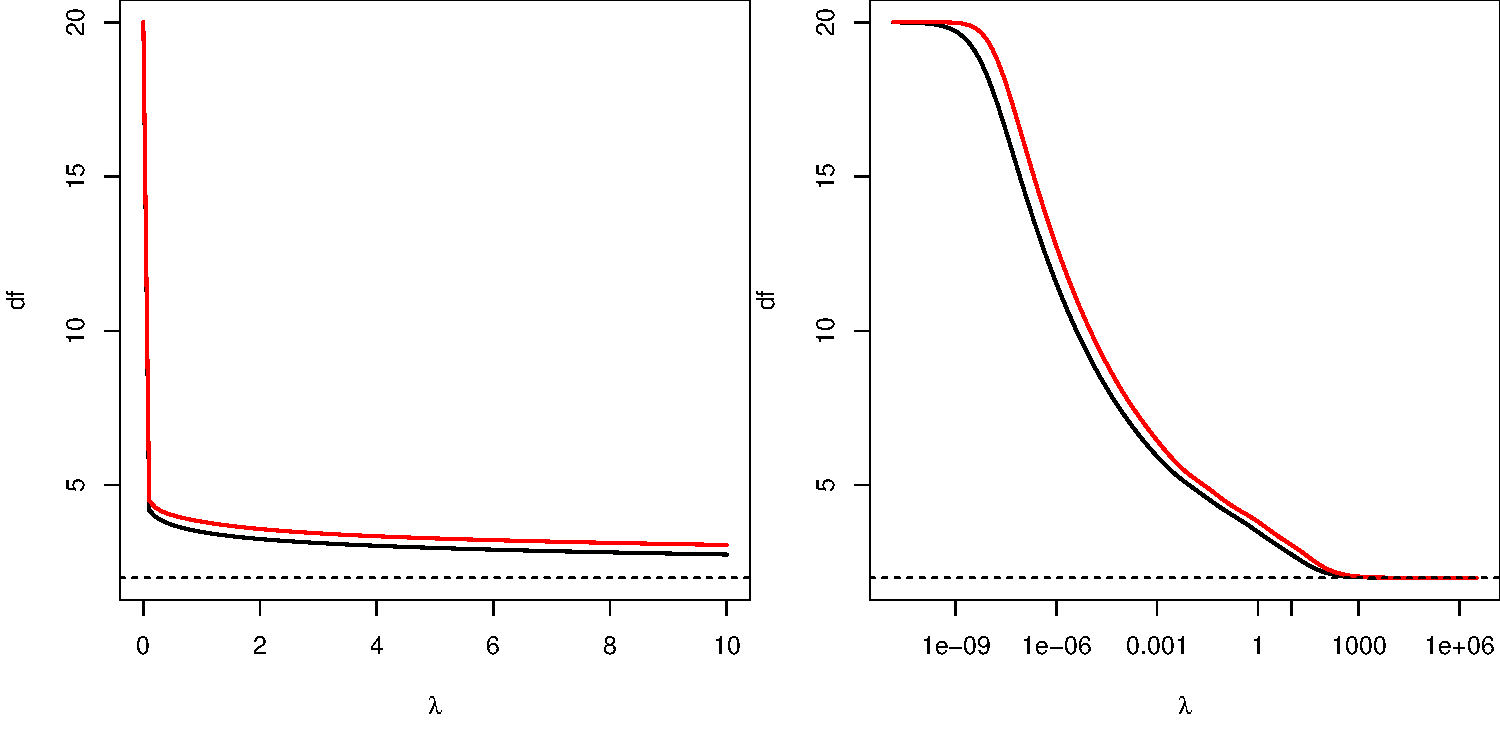
\includegraphics[width=0.9\textwidth]{figure/020-regression-1unnamed-chunk-35-1} 

}



\end{knitrout}



\end{frame}


\section[Basi]{Altre basi}

\begin{frame}[allowframebreaks=0.95]{Spline: diverse rappresentazioni}
\begin{itemize}
\item
In termini generali la rappresentazione \`e
\[ y_i = \beta_1+\sum_{k=1}^K b_kB_k(z_i) + \mbox{other variables} + \varepsilon_i\]
per un dato insieme di funzioni note $B_1,\ldots,B_K$ che \`e detta {\bf base}. 
\item
Questo fa s\`i che lo spazio di funzioni in cui cerchiamo un'approssimazione di $f$ contiene funzioni del tipo
\[ s(z) = \sum_{k=1}^K b_kB_k(z) \]
\item Ci sono diverse scelte di $B_k(z)$ che fan s\`i che si ottengano forme flessibili a partire da un numero ridotto di $B_k(z)$ (basso $K$),
\item una buona scelta di queste funzioni rende gli stimatori pi\`u efficienti.
\end{itemize}

%\break
%
%Non discutiamo oltre il problema della scelta delle basi, di seguito un tipico esempio
%
%<<echo=FALSE,out.width='0.95\\textwidth',out.height='0.4\\textwidth',fig.width=9,fig.height=4,cache=FALSE>>=
%library(splines)
%par(mfrow=c(1,2),mar=c(2,2,2,0.5),cex=1.4)
%xx=seq(0,1,length=100)
%BX=bs(xx,knots=seq(0,1,length=4))
%matplot(xx,BX,type="l",lwd=2,lty=1,main="Funzioni base")
%esempicurve=replicate(5,BX %*% rnorm(7,0,4))
%matplot(esempicurve[,1,],type="l",lwd=2,lty=1,col="blue",main="s()")
%@
%\begin{itemize}
%\item {\bf Sinistra:} funzioni base $B_k(\cdot)$;
%\item {\bf Destra:} cinque combinazioni linearei delle $B_k(\cdot)$ d sinistra.
%\end{itemize}
\end{frame}



\begin{frame}{Basi alternative}
La base a polinomi troncati \`e la pi\`u agevole da trattare dal punto di vista teorico, non \`e ottimale dal punto di vista computazionale.

\spazio

Il problema principale \`e che la matrice di disegno $X$ ha colonne fortemente correlate, il che pu\`o comportare instabilit\`a numerica.

\spazio

Esistono numerose alternative
\begin{itemize}
\item $B$-spline
\item $P$-spline
\item base radiale
\item $\ldots$
\end{itemize}

Si tenga presente che, in linea di principio, un cambio di base non comporta un cambiamento del modello.
\end{frame}

\begin{frame}[fragile,allowframebreaks=0.95]{B-spline: costruzione della base}
\begin{itemize}
\item siano $\tau_1 < \ldots < \tau_K$ i nodi interni;
\item sia $[a,b]$ il supporto di $x$ ($a<\tau_1$, $b>\tau_K$);
\item fissati, arbitrariamente, $\xi_1\leq \ldots \xi_M \leq a$ e $\chi_M\geq \ldots \geq \chi_1 \geq b$ (ad es. $\xi_i=a$ e $\nu_i=b$);
\item si ha allora la sequenza $\nu_1,\ldots,\nu_{K+2M}$.
\end{itemize}
\begin{center}
\begin{knitrout}
\definecolor{shadecolor}{rgb}{0.969, 0.969, 0.969}\color{fgcolor}
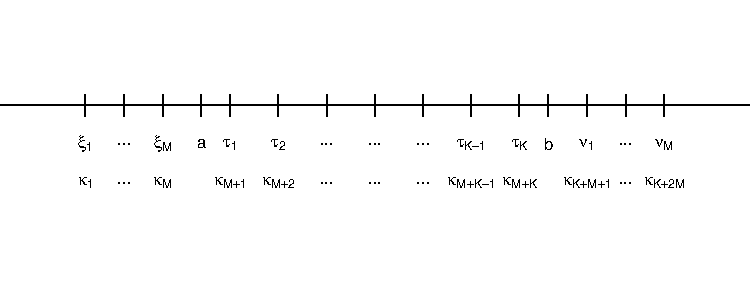
\includegraphics[width=0.8\textwidth]{figure/020-regression-1unnamed-chunk-36-1} 

\end{knitrout}
\end{center}

\break

Sia $B_{i,m}$ l'$i$-esima funzione base di ordine $m<M$, $i=1,\ldots, K+2M-m$, questa \`e definita ricorsivamente da
\[
B_{i,1}(x) = \begin{cases} 1 &\mbox{if }\nu_i\leq x < \nu_{i+1} \\ 0 & \mbox{altrimenti} \end{cases}
\]
per $i = 1,\ldots,K + 2M-1$ e
\[ 
B_{i,m}(x) = \frac{x-\nu_i}{\nu_{i+m-1}-\nu_i}B_{i,m-1}(x) +
\frac{\nu_{i+m}-x}{\nu_{i+m}-\nu_{i+1}}B_{i+1,m-1}(x)
\]
$i = 1,\ldots,K + 2M-m$.

Per $M=4$ si ottengono $K+4$ spline cubiche.


\end{frame}

\begin{frame}[fragile,allowframebreaks=0.95]{B-spline}
\begin{knitrout}
\definecolor{shadecolor}{rgb}{0.969, 0.969, 0.969}\color{fgcolor}\begin{kframe}


{\ttfamily\noindent\bfseries\color{errorcolor}{Error in eval(expr, envir, enclos): oggetto "{}lidar"{} non trovato}}\end{kframe}
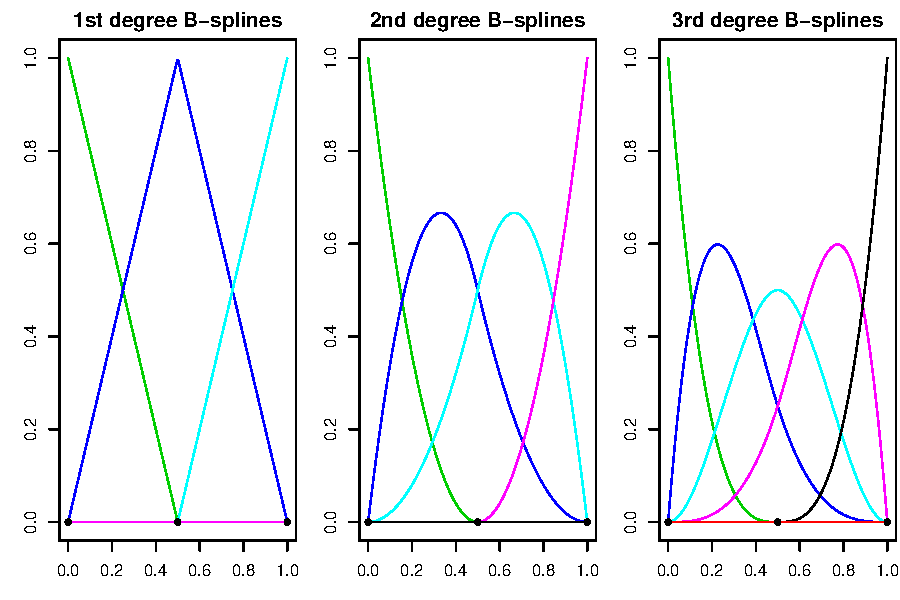
\includegraphics[width=0.8\textwidth,height=0.8\textheight]{figure/020-regression-1bsplineA-1} 

\end{knitrout}
\end{frame}

\begin{frame}{B-spline: penalty matrix}

Setting $M=4$, the penalty matrix is defined as
\[ \Omega_{ij} = \int_a^b B_i''(x)B_j''(x)dx  \]
Wand and Ormerod (2009) obtained formulas for calculating $\Omega$ in practice
\[ \Omega = (\tilde{B}'')^T \mbox{diag}(\mathbf w) \tilde{B}''  \]
where 
\[ [\tilde{B}'']_{ij} = \tilde{B}_j(\tilde{x}_i) \in\mathcal M_{3(K+7)\times(K+4)}\]
\[ \tilde{x} = \left(\nu_1,\frac{\nu_1+\nu_2}{2},\nu_2,\ldots,\nu_{K+7},\frac{\nu_{K+7}+\nu_{K+8}}{2},\nu_{k+8} \right) \]
\[ {\mathbf w} = \left(\frac{1}{6}(\Delta\nu)_1,\frac{4}{6}(\Delta\nu)_1,\frac{1}{6}(\Delta\nu)_1, \ldots, \frac{1}{6}(\Delta\nu)_{K+7},\frac{4}{6}(\Delta\nu)_{K+7},\frac{1}{6}(\Delta\nu)_{K+7}\right) \]
where $(\Delta\nu)_h=\nu_{h+1}-\nu_h$.
\end{frame}

\begin{frame}{P-spline}
Le $P$-spline sono costituite da
\begin{itemize}
\item una base di $B$-spline, di solito su nodi equidistanti
\item la penalizzazione
\[ \sum_{i=1}^{K-1} (b_{i+1}-b_i)^2 \]
ovvero
\[ {\bm b}^T 
\begin{bmatrix} 
1  & -1 & 0  & \cdot & \cdot \\ 
-1 &  2 & -1 & \cdot & \cdot \\
 0 & -1 &  2 & \cdot & \cdot \\
& \cdot& \cdot& \cdot& \cdot & \cdot \\
& \cdot& \cdot& \cdot& \cdot & \cdot \\
\end{bmatrix} 
{\bm b} \]
\end{itemize}
\end{frame}


\begin{frame}{Un esempio di $P$-spline}
\begin{columns}
\column{0.6\textwidth}
\begin{knitrout}
\definecolor{shadecolor}{rgb}{0.969, 0.969, 0.969}\color{fgcolor}
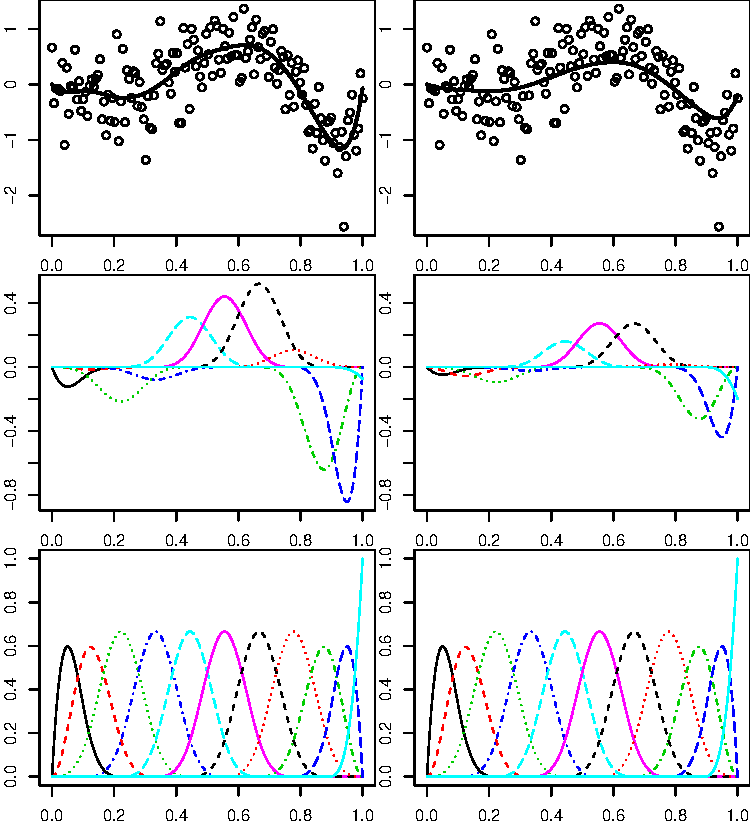
\includegraphics[width=0.95\textwidth]{figure/020-regression-1unnamed-chunk-37-1} 

\end{knitrout}
\column{0.4\textwidth}
Due $P$-spline, per quella a  sinistra
\[ \sum_{i=1}^{K-1} (b_{i+1}-b_i)^2= 4.39 \]
mentre per quella a destra
\[ \sum_{i=1}^{K-1} (b_{i+1}-b_i)^2= 0.92 \]
(pannello di mezzo: funzioni base moltiplicate per i rispettivi coefficienti, cio\`e la cui somma \`e la curva finale.)
\end{columns}
\end{frame}



\begin{frame}{Base radiale}
La base radiale di ordine $m$ con nodi $\nu_1,\ldots,\nu_K$ \`e
\[ 1, x, \ldots, x^m, B_k(x) = |x-\nu_k|^m \]
\begin{knitrout}
\definecolor{shadecolor}{rgb}{0.969, 0.969, 0.969}\color{fgcolor}\begin{kframe}


{\ttfamily\noindent\bfseries\color{errorcolor}{Error in eval(expr, envir, enclos): oggetto "{}lidar"{} non trovato}}\end{kframe}
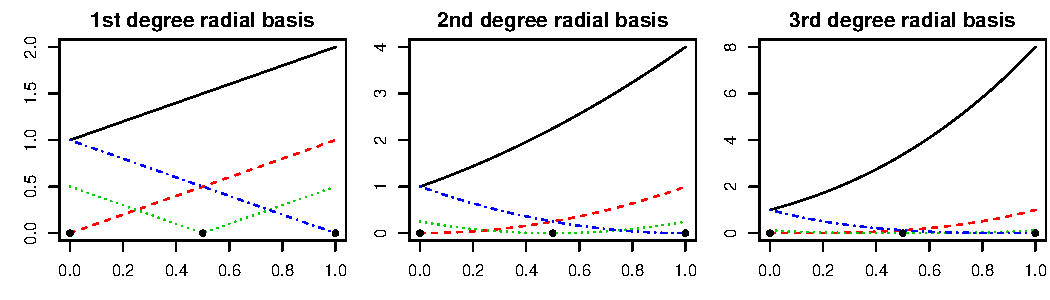
\includegraphics[width=0.8\textwidth]{figure/020-regression-1radialbasis-1} 

\end{knitrout}

Con matrice di penalizzazione
\[ [D]_{ij} = |\nu_i-\nu_j|^3 \]

\end{frame}




\section[Multiplo]{Pi\`u esplicative}

\begin{frame}{Pi\`u esplicative}
Supponiamo che le osservazioni includano pi\`u esplicative
\[ x_{i},z_{i},u_{i1},\ldots,u_{iq}  \]
Si possono ipotizzare diversi modelli
\begin{itemize}
\item componenti parametriche e una componente non parametrica
\[ y_i = {\bm\beta}^T{\bf u}_i + f(x_i) + \varepsilon_i \]
\item componenti parametriche e non parametriche
\[ y_i = {\bm\beta}^T{\bf u}_i + f_x(x_i) + f_z(z_i) + \varepsilon_i \]
\item componenti parametriche e non parametrica multipla
\[ y_i = {\bm\beta}^T{\bf u}_i + f(x_i,z_i) + \varepsilon_i \]
\end{itemize}
\end{frame}

\begin{frame}{Componenti parametriche e non parametrica}
Data per la spline $f$ la rappresentazione
\[ f(x_i) = b_0 + b_1 x_i + \sum_{j=1}^K B_j(x_i)b_{1+j} \]
con matrice di penalizzazione $S$ il modello
\[ y_i = {\bm\beta}^T{\bf u} + f(x_i) + \varepsilon_i \]
\`e stimato minimizzando la funzione obiettivo
\[ \sum_{i=1}^n(y_i - {\bm\beta}^T{\bf u}_i - f(x_i))^2 + \lambda{\bf b}^TS{\bf b} \]
in forma matriciale
\[ ||{\bm y} - H{\bm\theta}||^2 + \lambda{\bm\theta}^TS'{\bm\theta} \]
dove
\[ H=[U\; X],\;\;{\bm\theta}^T=({\bm\beta},{\bf b}),\;\;S'=? \]
\end{frame}

\begin{frame}{Componenti parametriche e non parametriche}
Siano le due spline $f_x$, $f_z$ rappresentate da
\[ f_x(x_i) = b_0 + b_1 x_i + \sum_{j=1}^{K_B} B_j(x_i)b_{1+j} \]
\[ f_z(z_i) = d_1 z_i + \sum_{j=1}^{K_D} D_j(z_i)d_{1+j} \]
con penalizzazioni $S_B, S_D$.

Si noti che la rappresentazione di $f_z$ non include l'intercetta per garantire l'identificabilit\`a del modello
\[ y_i = {\bm\beta}^T{\bf u}_i + f_x(x_i) + f_z(z_i) + \varepsilon_i \]
\end{frame}

\begin{frame}{Componenti parametriche e non parametriche}
Il modello
\[ y_i = {\bm\beta}^T{\bf u}_i + f_x(x_i) + f_z(z_i) + \varepsilon_i \]
\`e stimato minimizzando la funzione obiettivo
\[ \sum_{i=1}^n(y_i - {\bm\beta}^T{\bf u}_i - f_x(x_i)-f_z(z_i))^2 + \lambda{\bf b}^TS_x{\bf b}+ \lambda{\bf d}^TS_z{\bf d} \]
in forma matriciale
\[ ||{\bm y} - H{\bm\theta}||^2 + \lambda{\bf b}^TS_x{\bf b}+ \lambda{\bf d}^TS_z{\bf d} \]
dove
\[ H=[U\; X\; Z],\;\;{\bm\theta}^T=({\bm\beta},{\bf b},{\bf d})\]
\end{frame}

\begin{frame}{Componente non parametrica multivariata}
Il modello
\[ y_i = {\bm\beta}^T{\bf u}_i + f(x_i,z_i) + \varepsilon_i \]
richiede si definisca una spline bivariata.
\begin{itemize}
\item in linea di principio questo funziona allo stesso modo
\item {\bf problema della dimensionalit\`a}
\begin{itemize}
\item l'onere computazionale pu\`o crescere esponenzialmente con la dimensione
\item MSE: se il campione ha dimensione $n$ e la spline dimensione $d$ allora tipicamente
\[ \mbox{MSE} \approx \frac{c}{n^{4/(4+d)}} \]
cio\`e la numerosit\`a campionaria richiesta per mantenere l'MSE a un livello prespecificato cresce esponenzilmente con $d$:
\[ n \approx (c/\delta)^{d/4} \]
\end{itemize}
\end{itemize}
\end{frame}


\begin{frame}{Regressione non lineare in breve}
Dettagli tecnici a parte, i punti essenziali sono che
\begin{itemize}
\item 
possiamo specificare un modello per $y$ in cui
\[
\begin{matrix}
y_i &=& s(z_i) &+& \beta_0 + \beta_1 x_{i1} + \ldots + \beta_p x_{ip} &+& \varepsilon_i \\
y_i &=& s(z_i) &+&  \mbox{eff. lineari altre var.}                     &+& \mbox{error} 
\end{matrix}
\]
dove $s(\cdot)$ \`e una funzione liscia.
\item
disponiamo di strumenti per stimare $s(\cdot)$ con un prefissato grado di lisciamento (fix $K$, fix $\lambda$).
\item
disponiamo di strumenti per stimare $s(\cdot)$ con un grado di lisciamento ottimale.
\end{itemize}
Con questa strategia la forma della relazione tra $y$ e $z$ pu\`o essere qualunque (o quasi) senza bisogno di fare specifiche assunzioni.
\end{frame}


\section[GAM]{Modelli additivi generalizzati}

\begin{frame}{BPD data}
La displasia broncopolmonare (BPD) \`e una malattia tipica dei bambini nati prematuramente, la cui insorgenza \`e plausibilmente legata al peso alla nascita (birthweight).

\begin{columns}
\column{0.5\textwidth}
Per 223 bambini si \`e osservato
\begin{itemize}
\item birthweight
\item insorgenza di displasia broncopolmonare (BPD)
\end{itemize}
\column{0.5\textwidth}
\begin{knitrout}
\definecolor{shadecolor}{rgb}{0.969, 0.969, 0.969}\color{fgcolor}\begin{kframe}


{\ttfamily\noindent\bfseries\color{errorcolor}{Error in plot(bpd\$birthweight, bpd\$BPD, pch = "{}|"{}): oggetto "{}bpd"{} non trovato}}\end{kframe}
\end{knitrout}
\end{columns}

La v. risposta \`e dicotomica $\Rightarrow$ GLM.
\end{frame}

\begin{frame}[t]{Modelli additivi generalizzati}  
La generalizzazione a risposta non gaussiana funziona in modo analogo all'estensione da ML  a GLM.
\onslide*<1>{
\[
\begin{array}{ccc}
\mbox{LM} & \rightarrow & \mbox{GLM} \\
Y_i\thicksim\mathcal N(\mu_i,\sigma^2) 
& &
Y_i\thicksim\mbox{Expon}(\theta_i,\phi_i)
\\
E(Y_i) = \eta_i
& &
g(E(Y_i)) = \eta_i
\\
\eta_i = \mu_i = {\bf x}_i {\bm\beta}
& &
\eta_i = {\bf x}_i {\bm\beta}
\\
\end{array}
\]

\[
\begin{array}{ccc}
\mbox{AM} & \rightarrow & \mbox{GAM} \\
Y_i\thicksim\mathcal N(\mu_i,\sigma^2) 
& &
Y_i\thicksim\mbox{Expon}(\theta_i,\phi_i)
\\
E(Y_i) = \eta_i
& &
g(E(Y_i)) = \eta_i
\\
\eta_i = \mu_i = f(x_i)
& &
\eta_i = f(x_i)
\\
\end{array}
\]
}
\onslide*<2>{
Data una spline
\[
f(x) = \beta_1+\beta_2 x + \sum_{j=1}^K \beta_{1+j}B_j(x)
\]
il criterio dei minimi quadrati penalizzati
\[  \sum_{i=1}^n (y_i-f(x_i))^2 + \lambda S(f(x)) \]
diventa il criterio della verosimiglianza penalizzata
\[  \ell({\bf \beta},{\bf b},\phi) - \lambda S(f(x)) \]
}
dove 
\[
 \ell({\bf \beta},{\bf b},\phi) = \sum_{i=1}^n \log(p(y_i;\theta_i))
  = \sum_{i=1}^n (y_i\theta_i-r_i(\theta_i)))/\phi + c(\phi;y_i)
\]
\end{frame}

\begin{frame}{P-IRLS}
In termini pratici si usa poi l'algoritmo IRLS usato nei GLM, con passo $k$
\begin{itemize}
\item[1] calcolare pseudodati
\[ z_i^{[k]} = g'(\mu_i^{[k]})(y_i-\mu_i^{[k]}) + \eta_i^{[k]} \]
e la matrice diagonale dei pesi
\[ W_{ii}^{[k]} = \frac{1}{V(\mu_i^{[k]})g'(\mu_i^{[k]})^2}\]
\item[2] porre
\[
{\bm\beta}^{[k+1]} \leftarrow 
\underset{{\bm{\beta}}}{\mbox{argmin}} \left\Vert\sqrt{W^{[k]}} ({\bf z}^{[k]}-X{\bm\beta})\right\Vert^2
\]
\end{itemize}

In un modello additivo la funzione obiettivo nel secondo passo \`e
\[
{\bm\beta}^{[k+1]} \leftarrow 
\underset{{\bm{\beta}}}{\mbox{argmin}} \left\Vert\sqrt{W^{[k]}} ({\bf z}^{[k]}-X{\bm\beta})\right\Vert^2
 + \lambda {\bm\beta}^TS{\bm\beta}\]
\end{frame}

\subsection{Scelta di $\lambda$ con dati non Gaussiani}

\begin{frame}{Errore di previsione  con dati non Gaussiani}
Con dati Gaussiani, la scelta di $\lambda$ \`e basata sulla stima dell'errore
\[ \sum_{i=1}^n (\hat{f}(x_i)-y_i)^2 \]
ottenuta via CV, da cui il criterio del GCV (per via della lineari\`a delle spline come lisciatori).

\spazio

La stessa strategia pu\`o essere usata ora {\bf ma} il lisciatore non \`e lineare, quindi il GCV e le derivazioni teoriche sono approssimate.

\end{frame}


\begin{frame}[t]{GCV per i GAM}
L'obiettivo nella stima GAM pu\`o essere scritto
\onslide*<1>{in termini della devianza 
\[ D({\bm\beta})=2(\ell({\bm\beta}_{\mbox{max}})-\ell({\bm\beta})) \]
}
come
\[ D({\bm\beta})+\sum_{j=1}^d\lambda_j{\bm\beta}^TS_j{\bm\beta} \]
la cui approssimazione quadratica \`e, per un $\lambda$ fissato,
\[
\left\Vert\sqrt{W} ({\bf z}-X{\bm\beta})\right\Vert^2 + \sum_{j=1}^d\lambda_j{\bm\beta}^TS_j{\bm\beta}
\]
\onslide*<2->{
da cui il GCV (valido localmente)
\onslide<3>{ e quindi il GCV applicabile globalmente}
\[
\frac{n\left\Vert\sqrt{W} ({\bf z}-X{\bm\beta})\right\Vert^2}{n-\mbox{tr}(L)}
\onslide*<3>{\;\;\;\;\rightarrow\;\;\;\; \frac{nD({\bm\hat\beta})}{n-\mbox{tr}(L)}}
\]
}
\end{frame}


\begin{frame}{UBRE}
Ricordando che la CV nasce dal rischio di previsione, $E((m(x)-\hat{m}(x))^2)$, cio\`e
\[ E\left(\left\Vert{\bm\mu}-L{\bf y}\right\Vert^2\right)
=\frac{1}{n}E\left(\left\Vert{\bf y}-L{\bf y}\right\Vert^2\right) - \sigma^2 + 2\mbox{tr}(L)\frac{\sigma^2}{n}
\]
dove il parametro di scala $\sigma^2$ \`e noto si pu\`o impiegare l'UBRE (Unbiased Risk Estimator)
\[ \frac{1}{n}\left\Vert{\bf y}-L{\bf y}\right\Vert^2 - \sigma^2 + 2\mbox{tr}(L)\frac{\sigma^2}{n}
\]

\spazio

L'UBRE \`e appropriato per i GAM in cui il parametro di scala \`e noto.
\end{frame}

\begin{frame}{Calcolo dell'UBRE}
A partire da
\[ D({\bm\beta})+\sum_{j=1}^d\lambda_j{\bm\beta}^TS_j{\bm\beta} \]
e dall'approssimazione quadratica
\[
\left\Vert\sqrt{W} ({\bf z}-X{\bm\beta})\right\Vert^2 + \sum_{j=1}^d\lambda_j{\bm\beta}^TS_j{\bm\beta}
\]
si ottiene il criterio UBRE
\[
\frac{1}{n}\left\Vert\sqrt{W} ({\bf z}-X{\bm\beta})\right\Vert^2 -\sigma^2 + \frac{2\sigma^2}{n}\mbox{tr}(L)
\]
\[
\frac{1}{n}D({\bm\hat\beta}) -\sigma^2 + \frac{2\sigma^2}{n}\mbox{tr}(L)
\]
\end{frame}

\begin{frame}[fragile]{BPD data - modello stimato}

\begin{knitrout}
\definecolor{shadecolor}{rgb}{0.969, 0.969, 0.969}\color{fgcolor}\begin{kframe}
\begin{alltt}
\hlstd{fit}\hlkwb{=}\hlkwd{gam}\hlstd{(BPD}\hlopt{~}\hlkwd{s}\hlstd{(birthweight),}
        \hlkwc{data}\hlstd{=bpd,}
        \hlkwc{family}\hlstd{=binomial)}
\hlkwd{plot}\hlstd{(fit)}
\end{alltt}
\end{kframe}
\end{knitrout}

\begin{center}
\begin{knitrout}
\definecolor{shadecolor}{rgb}{0.969, 0.969, 0.969}\color{fgcolor}\begin{kframe}


{\ttfamily\noindent\bfseries\color{errorcolor}{Error in is.data.frame(data): oggetto "{}bpd"{} non trovato}}\end{kframe}
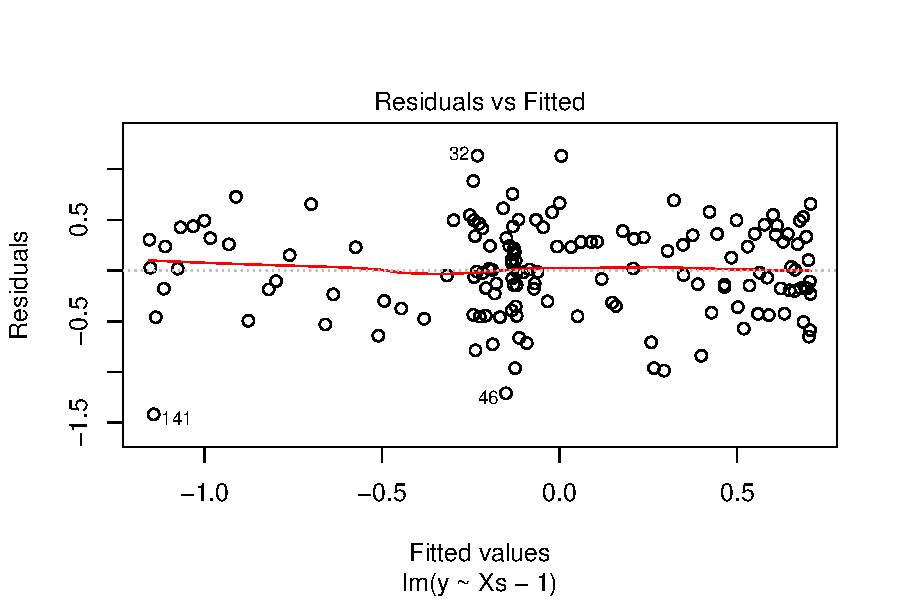
\includegraphics[width=0.7\textwidth]{figure/020-regression-1unnamed-chunk-40-1} 

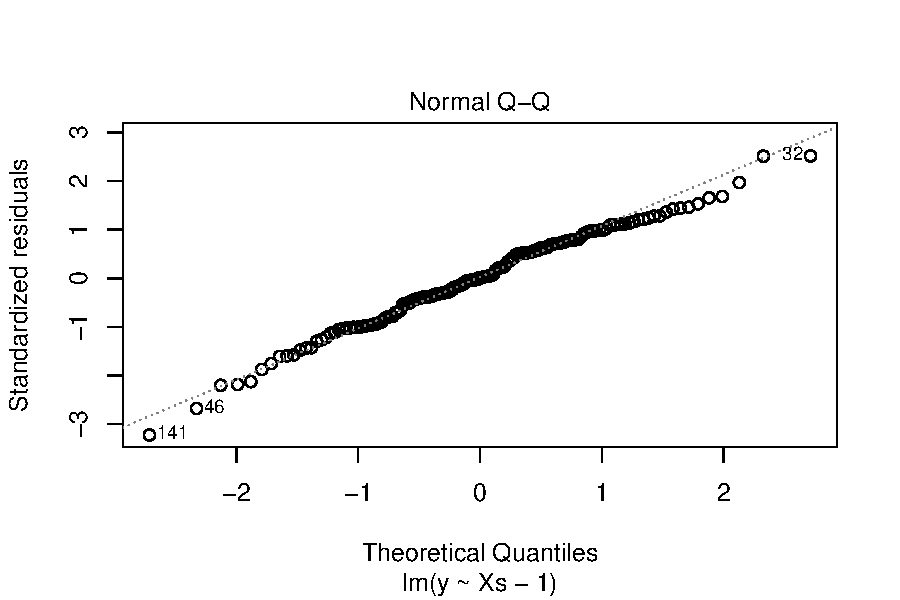
\includegraphics[width=0.7\textwidth]{figure/020-regression-1unnamed-chunk-40-2} 

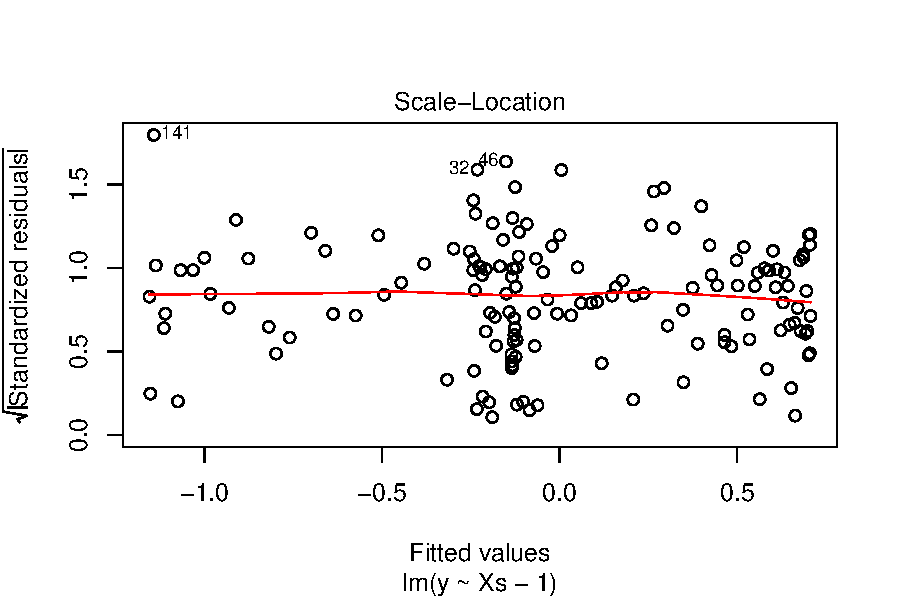
\includegraphics[width=0.7\textwidth]{figure/020-regression-1unnamed-chunk-40-3} 

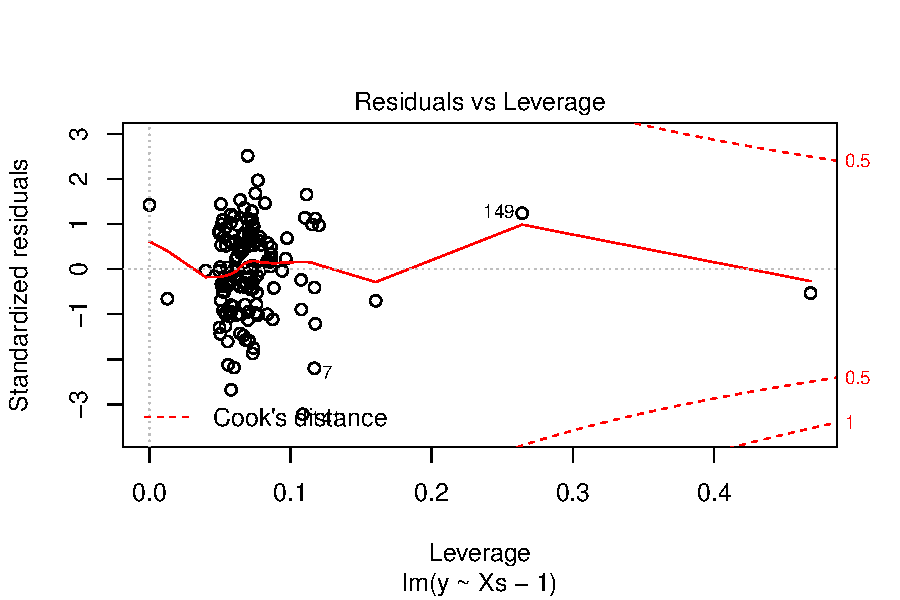
\includegraphics[width=0.7\textwidth]{figure/020-regression-1unnamed-chunk-40-4} 

\end{knitrout}
\end{center}

\end{frame}


\begin{frame}[fragile]{BPD data - modello stimato}

\begin{center}
\begin{knitrout}
\definecolor{shadecolor}{rgb}{0.969, 0.969, 0.969}\color{fgcolor}\begin{kframe}
\begin{alltt}
\hlkwd{curve}\hlstd{(}\hlkwd{predict}\hlstd{(fit,}\hlkwc{newdata}\hlstd{=}\hlkwd{data.frame}\hlstd{(}\hlkwc{birthweight}\hlstd{=x)),}
      \hlkwc{from}\hlstd{=}\hlnum{400}\hlstd{,}\hlkwc{to}\hlstd{=}\hlnum{1800}\hlstd{,}\hlkwc{ylab}\hlstd{=}\hlstr{""}\hlstd{)}
\end{alltt}


{\ttfamily\noindent\color{warningcolor}{Warning: 'newdata' had 101 rows but variables found have 150 rows}}

{\ttfamily\noindent\bfseries\color{errorcolor}{Error in curve(predict(fit, newdata = data.frame(birthweight = x)), from = 400, : 'expr' did not evaluate to an object of length 'n'}}\begin{alltt}
\hlkwd{rug}\hlstd{(bpd}\hlopt{$}\hlstd{birthweight[bpd}\hlopt{$}\hlstd{BPD}\hlopt{==}\hlnum{0}\hlstd{],}\hlkwc{side}\hlstd{=}\hlnum{1}\hlstd{)}
\end{alltt}


{\ttfamily\noindent\bfseries\color{errorcolor}{Error in as.vector(x): oggetto "{}bpd"{} non trovato}}\begin{alltt}
\hlkwd{rug}\hlstd{(bpd}\hlopt{$}\hlstd{birthweight[bpd}\hlopt{$}\hlstd{BPD}\hlopt{==}\hlnum{1}\hlstd{],}\hlkwc{side}\hlstd{=}\hlnum{3}\hlstd{)}
\end{alltt}


{\ttfamily\noindent\bfseries\color{errorcolor}{Error in as.vector(x): oggetto "{}bpd"{} non trovato}}\end{kframe}
\end{knitrout}
\end{center}

\end{frame}

\begin{frame}[fragile]{BPD data - modello stimato}

\begin{center}
\begin{scriptsize}
\begin{knitrout}
\definecolor{shadecolor}{rgb}{0.969, 0.969, 0.969}\color{fgcolor}\begin{kframe}
\begin{alltt}
\hlkwd{curve}\hlstd{(}\hlkwd{predict}\hlstd{(fit,}\hlkwc{newdata}\hlstd{=}\hlkwd{data.frame}\hlstd{(}\hlkwc{birthweight}\hlstd{=x),}
              \hlkwc{type}\hlstd{=}\hlstr{"response"}\hlstd{),}
      \hlkwc{from}\hlstd{=}\hlnum{400}\hlstd{,}\hlkwc{to}\hlstd{=}\hlnum{1800}\hlstd{,}\hlkwc{ylab}\hlstd{=}\hlstr{""}\hlstd{)}
\end{alltt}


{\ttfamily\noindent\color{warningcolor}{Warning: 'newdata' had 101 rows but variables found have 150 rows}}

{\ttfamily\noindent\bfseries\color{errorcolor}{Error in curve(predict(fit, newdata = data.frame(birthweight = x), type = "{}response"{}), : 'expr' did not evaluate to an object of length 'n'}}\begin{alltt}
\hlkwd{rug}\hlstd{(bpd}\hlopt{$}\hlstd{birthweight[bpd}\hlopt{$}\hlstd{BPD}\hlopt{==}\hlnum{0}\hlstd{],}\hlkwc{side}\hlstd{=}\hlnum{1}\hlstd{)}
\end{alltt}


{\ttfamily\noindent\bfseries\color{errorcolor}{Error in as.vector(x): oggetto "{}bpd"{} non trovato}}\begin{alltt}
\hlkwd{rug}\hlstd{(bpd}\hlopt{$}\hlstd{birthweight[bpd}\hlopt{$}\hlstd{BPD}\hlopt{==}\hlnum{1}\hlstd{],}\hlkwc{side}\hlstd{=}\hlnum{3}\hlstd{)}
\end{alltt}


{\ttfamily\noindent\bfseries\color{errorcolor}{Error in as.vector(x): oggetto "{}bpd"{} non trovato}}\end{kframe}
\end{knitrout}
\end{scriptsize}
\end{center}

\end{frame}

\begin{frame}[fragile]{BPD data - modello stimato}

\begin{center}
\begin{scriptsize}
\begin{knitrout}
\definecolor{shadecolor}{rgb}{0.969, 0.969, 0.969}\color{fgcolor}\begin{kframe}
\begin{alltt}
\hlstd{xx}\hlkwb{=}\hlkwd{seq}\hlstd{(}\hlnum{450}\hlstd{,}\hlnum{1730}\hlstd{,}\hlkwc{length}\hlstd{=}\hlnum{100}\hlstd{)}
\hlstd{pr}\hlkwb{=}\hlkwd{predict}\hlstd{(fit,}\hlkwc{newdata}\hlstd{=}\hlkwd{data.frame}\hlstd{(}\hlkwc{birthweight}\hlstd{=xx),}
              \hlkwc{type}\hlstd{=}\hlstr{"response"}\hlstd{,}\hlkwc{se.fit}\hlstd{=}\hlnum{TRUE}\hlstd{)}
\end{alltt}


{\ttfamily\noindent\color{warningcolor}{Warning: 'newdata' had 100 rows but variables found have 150 rows}}\begin{alltt}
\hlkwd{matplot}\hlstd{(xx,}\hlkwd{cbind}\hlstd{(pr}\hlopt{$}\hlstd{fit}\hlopt{-}\hlnum{2}\hlopt{*}\hlstd{pr}\hlopt{$}\hlstd{se.fit,pr}\hlopt{$}\hlstd{fit,pr}\hlopt{$}\hlstd{fit}\hlopt{+}\hlnum{2}\hlopt{*}\hlstd{pr}\hlopt{$}\hlstd{se.fit),}
        \hlkwc{type}\hlstd{=}\hlstr{"l"}\hlstd{,}\hlkwc{lty}\hlstd{=}\hlkwd{c}\hlstd{(}\hlnum{2}\hlstd{,}\hlnum{1}\hlstd{,}\hlnum{2}\hlstd{),}\hlkwc{col}\hlstd{=}\hlstr{"black"}\hlstd{)}
\end{alltt}


{\ttfamily\noindent\bfseries\color{errorcolor}{Error in matplot(xx, cbind(pr\$fit - 2 * pr\$se.fit, pr\$fit, pr\$fit + 2 * : 'x' and 'y' must have same number of rows}}

{\ttfamily\noindent\bfseries\color{errorcolor}{Error in as.vector(x): oggetto "{}bpd"{} non trovato}}

{\ttfamily\noindent\bfseries\color{errorcolor}{Error in as.vector(x): oggetto "{}bpd"{} non trovato}}\end{kframe}
\end{knitrout}
\end{scriptsize}
\end{center}

\end{frame}

\begin{frame}[fragile]{BPD data - modello stimato}

\begin{center}
\begin{scriptsize}
\begin{knitrout}
\definecolor{shadecolor}{rgb}{0.969, 0.969, 0.969}\color{fgcolor}\begin{kframe}
\begin{alltt}
\hlstd{xx}\hlkwb{=}\hlkwd{seq}\hlstd{(}\hlnum{450}\hlstd{,}\hlnum{1730}\hlstd{,}\hlkwc{length}\hlstd{=}\hlnum{100}\hlstd{)}
\hlstd{pr}\hlkwb{=}\hlkwd{predict}\hlstd{(fit,}\hlkwc{newdata}\hlstd{=}\hlkwd{data.frame}\hlstd{(}\hlkwc{birthweight}\hlstd{=xx),}
              \hlkwc{se.fit}\hlstd{=}\hlnum{TRUE}\hlstd{)}
\end{alltt}


{\ttfamily\noindent\color{warningcolor}{Warning: 'newdata' had 100 rows but variables found have 150 rows}}\begin{alltt}
\hlkwd{matplot}\hlstd{(xx,}\hlkwd{cbind}\hlstd{(pr}\hlopt{$}\hlstd{fit}\hlopt{-}\hlnum{2}\hlopt{*}\hlstd{pr}\hlopt{$}\hlstd{se.fit,pr}\hlopt{$}\hlstd{fit,pr}\hlopt{$}\hlstd{fit}\hlopt{+}\hlnum{2}\hlopt{*}\hlstd{pr}\hlopt{$}\hlstd{se.fit),}
        \hlkwc{type}\hlstd{=}\hlstr{"l"}\hlstd{,}\hlkwc{lty}\hlstd{=}\hlkwd{c}\hlstd{(}\hlnum{2}\hlstd{,}\hlnum{1}\hlstd{,}\hlnum{2}\hlstd{),}\hlkwc{col}\hlstd{=}\hlstr{"black"}\hlstd{)}
\end{alltt}


{\ttfamily\noindent\bfseries\color{errorcolor}{Error in matplot(xx, cbind(pr\$fit - 2 * pr\$se.fit, pr\$fit, pr\$fit + 2 * : 'x' and 'y' must have same number of rows}}

{\ttfamily\noindent\bfseries\color{errorcolor}{Error in as.vector(x): oggetto "{}bpd"{} non trovato}}

{\ttfamily\noindent\bfseries\color{errorcolor}{Error in as.vector(x): oggetto "{}bpd"{} non trovato}}\end{kframe}
\end{knitrout}
\end{scriptsize}
\end{center}

\end{frame}



\end{document}





